\id{МРНТИ 20.01.00}; 20.15.05

{\bfseries ИННОВАЦИОННЫЕ АРХИТЕКТУРНЫЕ РЕШЕНИЯ И МЕЖДИСЦИПЛИНАРНАЯ
РЕАЛИЗАЦИЯ ОБЛАЧНОЙ ПЛАТФОРМЫ BULT ДЛЯ ОРКЕСТРАЦИИ ВЕБ-ПРИЛОЖЕНИЙ}

{\bfseries \textsuperscript{1}A.К. Шайханова}
\begin{figure}[H]
	\centering
	
\includegraphics[width=0.8\textwidth]{media/ict/image1}
	\caption*{}
\end{figure}

\textsuperscript{2}Ж.А. Бермухамбетов}
\begin{figure}[H]
	\centering
	
\includegraphics[width=0.8\textwidth]{media/ict/image1}
	\caption*{}
\end{figure}

Ким}
\begin{figure}[H]
	\centering
	
\includegraphics[width=0.8\textwidth]{media/ict/image1}
	\caption*{}
\end{figure}

{\bfseries \textsuperscript{3}А.О.
\begin{figure}[H]
	\centering
	
\includegraphics[width=0.8\textwidth]{media/ict/image1}
	\caption*{}
\end{figure}


\emph{\textsuperscript{1}Евразийский национальный университет имени Л.Н.
Гумилева, Астана, Казахстан,}

\emph{\textsuperscript{2} ТОО «WebTotem», Астана, Казахстан,}

\emph{\textsuperscript{3}Astana IT University, Астана, Казахстан}

{\bfseries \textsuperscript{\envelope }}Корреспондент-автор:
\href{mailto:Arailym.tll@gmail.com}{\nolinkurl{Arailym.tll@gmail.com}}

Статья посвящена созданию облачной платформы BULT, которая реализует
междисциплинарный подход к разработке и оркестрации веб-приложений.
Основной целью данной работы является разработка платформы,
обеспечивающей гибкость, масштабируемость и интеграцию различных
технологий. Описаны архитектурные решения, включающие микросервисную
архитектуру и контейнеризацию, что упрощает развертывание и управление
приложениями. В качестве основы для оркестрации контейнеров используется
Nomad от HashiCorp, который позволяет динамически управлять
распределением задач и ресурсов, обеспечивая эффективность и
устойчивость работы приложений. Система управления данными реализована
на базе PostgreSQL и JuiceFS, что обеспечивает высокую
производительность и надежность хранения данных. Для обеспечения
безопасности используются Wireguard и Let' s Encrypt,
обеспечивающие шифрование сетевого трафика и автоматическое обновление
SSL-сертификатов. Мониторинг и анализ системы осуществляются с помощью
Grafana и Loki, позволяющих визуализировать метрики и логи в реальном
времени. Внедрение принципов DevOps и автоматизация процессов
разработки, тестирования и развертывания достигаются с использованием
инструментов CI/CD, что позволяет быстро и безопасно внедрять изменения
и новые функции. Применение междисциплинарного подхода позволяет
учитывать различные аспекты разработки и эксплуатации систем, что делает
платформу BULT конкурентоспособным решением на современном рынке
облачных технологий, обеспечивая высокую производительность, надежность
и удобство эксплуатации веб-приложений. Приведены примеры практического
применения платформы и её преимущества в сравнении с традиционными
подходами.

{\bfseries Ключевые слова:} облачная платформа, междисциплинарный подход,
веб-приложения, оркестрация, инновационные методы, контейнеризация,
безопасность данных, автоматизация процессов{\bfseries .}

{\bfseries ИННОВАЦИЯЛЫҚ АРХИТЕКТУРАЛЫҚ ШЕШІМДЕР ЖӘНЕ ВЕБ-ҚОСЫМШАЛАРДЫ
ОРКЕСТРЛЕУГЕ АРНАЛҒАН BULT БҰЛТТЫ ПЛАТФОРМАСЫН ПӘНАРАЛЫҚ ЕНГІЗУ}

{\bfseries \textsuperscript{1}A.К. Шайханова, \textsuperscript{2}Ж.А.
Бермухамбетов, \textsuperscript{2}В.В. Ким, \textsuperscript{3}А.О.
Тлеубаева\textsuperscript{\envelope }}

\emph{\textsuperscript{1}Л.Н. Гумилев атындағы Еуразия ұлттық
университеті, Астана, Қазақстан,}

\emph{\textsuperscript{2} «WebTotem» ЖШС, Астана, Қазақстан,}

\emph{\textsuperscript{3}Astana IT University, Астана, Қазақстан,}

\emph{e-mail:
\href{mailto:Arailym.tll@gmail.com}{\nolinkurl{Arailym.tll@gmail.com}}}

Мақала веб-қосымшаларды әзірлеу мен оркестрлеудің пәнаралық тәсілін
жүзеге асыратын BULT бұлтты платформасын құруға бағытталған. Бұл
жұмыстың негізгі мақсаты әртүрлі технологиялардың икемділігін,
ауқымдылығын және интеграциясын қамтамасыз ететін платформаны әзірлеу
болып табылады. Микросервистік архитектура мен контейнерлеуді қамтитын
архитектуралық шешімдер сипатталған, бұл қосымшаларды орналастыруды және
басқаруды жеңілдетеді. Контейнерлерді оркестрлеудің негізі ретінде
hashicorp '{} s Nomad қолданылады, ол қосымшалардың
тиімділігі мен тұрақтылығын қамтамасыз ете отырып, тапсырмалар мен
ресурстарды бөлуді динамикалық басқаруға мүмкіндік береді. Деректерді
басқару жүйесі PostgreSQL және JuiceFS негізінде жүзеге асырылады, бұл
деректерді сақтаудың жоғары өнімділігі мен сенімділігін қамтамасыз
етеді. Қауіпсіздік үшін желілік трафикті шифрлауды және SSL
сертификаттарын автоматты түрде жаңартуды қамтамасыз ететін Wireguard
және let '{} s Encrypt қолданылады. Жүйені бақылау және
талдау нақты уақыттағы көрсеткіштер мен журналдарды визуализациялауға
мүмкіндік беретін Grafana және Loki көмегімен жүзеге асырылады. DevOps
принциптерін енгізу және әзірлеу, тестілеу және орналастыру процестерін
автоматтандыру ci/CD құралдарын қолдану арқылы жүзеге асырылады, бұл
өзгерістер мен жаңа мүмкіндіктерді жылдам және қауіпсіз енгізуге
мүмкіндік береді. Пәнаралық тәсілді қолдану жүйелерді әзірлеу мен
пайдаланудың әртүрлі аспектілерін ескеруге мүмкіндік береді, бұл bult
платформасын веб-қосымшалардың жоғары өнімділігін, сенімділігін және
ыңғайлылығын қамтамасыз ететін заманауи бұлттық технологиялар нарығында
бәсекеге қабілетті ШЕШІМ ЕТЕДІ. Платформаны практикалық қолдану
мысалдары және оның дәстүрлі тәсілдермен салыстырғанда артықшылықтары
келтірілген.

{\bfseries Түйін сөздер:} бұлтты платформа, пәнаралық тәсіл,
веб-қосымшалар, оркестрация, инновациялық әдістер, контейнерлеу,
деректер қауіпсіздігі, процестерді автоматтандыру.

{\bfseries INNOVATIVE ARCHITECTURAL SOLUTIONS AND INTERDISCIPLINARY
IMPLEMENTATION OF THE BULT CLOUD PLATFORM FOR WEB APPLICATION
ORCHESTRATION}

{\bfseries \textsuperscript{1}A.K. Shaikhanova, \textsuperscript{2}Zh.A.}
{\bfseries Bermukhambetov, \textsuperscript{2}V.V. Kim,
\textsuperscript{3}A.O. Tleubayeva\textsuperscript{\envelope }}

\emph{\textsuperscript{1}L.N. Gumilyov Eurasian National University,
Astana, Kazakhstan,}

\emph{\textsuperscript{2} «WebTotem» LLP, Astana, Kazakhstan,}

\emph{\textsuperscript{3}Astana IT University, Astana, Kazakhstan,}

\emph{e-mail:
\href{mailto:Arailym.tll@gmail.com}{\nolinkurl{Arailym.tll@gmail.com}}}

The article is devoted to the creation of the BULT cloud platform, which
implements an interdisciplinary approach to the development and
orchestration of web applications. The main goal of this work is to
develop a platform that provides flexibility, scalability and
integration of various technologies. Architectural solutions including
microservice architecture and containerization are described, which
simplifies the deployment and management of applications.
HashiCorp' s Nomad is used as the basis for container
orchestration, which allows you to dynamically manage the distribution
of tasks and resources, ensuring the efficiency and stability of
applications. The data management system is implemented on the basis of
PostgreSQL and JuiceFS, which ensures high performance and reliability
of data storage. To ensure security, Wireguard and Let' s
Encrypt are used, which provide encryption of network traffic and
automatic updating of SSL certificates. Monitoring and analysis of the
system are carried out using Grafana and Loki, which allow you to
visualize metrics and logs in real time. The implementation of DevOps
principles and automation of development, testing and deployment
processes are achieved using CI/CD tools, which allows you to quickly
and safely implement changes and new features. The application of an
interdisciplinary approach allows us to take into account various
aspects of system development and operation, which makes the BULT
platform a competitive solution in the modern cloud technology market,
providing high performance, reliability and ease of use of web
applications. Examples of the practical application of the platform and
its advantages in comparison with traditional approaches are given.

{\bfseries Keywords:} cloud platform, interdisciplinary approach, web
applications, orchestration, innovative methods, containerization, data
security, process automation.

{\bfseries Введение.} Облачные технологии стали неотъемлемой частью
современных ИТ-систем, предоставляя организациям возможность гибкого и
масштабируемого управления ресурсами. С увеличением популярности
облачных решений возникают новые вызовы, связанные с их разработкой и
интеграцией. Одной из ключевых проблем является необходимость
объединения различных дисциплин, таких как программная инженерия,
безопасность данных, управление инфраструктурой и DevOps, в рамках
единой платформы. Это требует создания междисциплинарных архитектурных
решений, которые эффективно интегрируют данные технологии и обеспечивают
стабильную и надежную работу веб-приложений.

Актуальность данной работы обусловлена необходимостью решения
современных вызовов, с которыми сталкиваются разработчики облачных
платформ. В условиях постоянно возрастающей нагрузки на
ИТ-инфраструктуру первостепенное значение приобретают задачи обеспечения
высокой производительности, надежности и безопасности. Современные
исследования подтверждают важность междисциплинарного подхода для
решения этих задач. Например, Эберхард Вольф в своей книге
«Microservices: Architecting for Continuous Delivery and DevOps»
отмечает, что микросервисная архитектура является ключевым элементом для
обеспечения гибкости и производительности в условиях динамически
изменяющихся нагрузок в облачных средах {[}1{]}. В статье,
опубликованной в IEEE Software, рассматриваются основные вызовы, с
которыми сталкиваются разработчики при внедрении микросервисных
архитектур, что подчеркивает необходимость комплексного подхода к их
реализации {[}2{]}.

Кроме того, использование контейнеризации для повышения
производительности облачных приложений подробно обсуждается в
исследовании, опубликованном в IEEE Access, где описываются преимущества
контейнерных технологий для управления ресурсами в облачных платформах
{[}3{]}. Однако, с внедрением микросервисов и контейнеризации возникают
новые проблемы, связанные с безопасностью. В статье, опубликованной в
ACM Computing Surveys, рассматриваются ключевые аспекты безопасности в
микросервисных архитектурах и предлагаются стратегии по их преодолению
{[}4{]}.

Новизна данной работы заключается в разработке платформы BULT, которая
объединяет передовые технологии, такие как микросервисная архитектура и
контейнеризация, с целью создания более эффективных и надежных систем. В
отличие от существующих решений, BULT предлагает интеграцию таких
технологий, как Nomad от HashiCorp для оркестрации контейнеров, что
позволяет динамически управлять ресурсами и задачами с учетом их
изменяющихся требований. Это обеспечивает более высокую устойчивость и
производительность приложений в условиях переменных нагрузок.

Научная значимость исследования заключается в демонстрации того, как
интеграция различных дисциплин и технологий может улучшить процессы
разработки и эксплуатации облачных систем. Платформа BULT является
примером успешной реализации междисциплинарного подхода, который не
только повышает производительность и надежность веб-приложений, но и
обеспечивает гибкость управления ресурсами и защиту данных. Полученные
результаты могут быть использованы в дальнейшем для разработки
аналогичных систем в других областях, что делает это исследование
значимым как для академического сообщества, так и для индустрии.

Облачные платформы для разработки и оркестрации веб-приложений
становятся ключевыми элементами современных ИТ-инфраструктур,
предоставляя организациям возможность гибкого и масштабируемого
управления ресурсами. Одной из главных тенденций в этой области является
внедрение микросервисной архитектуры и контейнеризации, которые
позволяют разбивать приложения на независимые сервисы, что значительно
улучшает их гибкость и масштабируемость. Однако, несмотря на эти
преимущества, контейнеризации также связано с новыми рисками, такими как
необходимость в специфических подходах к обеспечению безопасности и
мониторингу {[}5{]}.

Kubernetes и OpenShift, как наиболее популярные платформы для
оркестрации контейнеров, предоставляют мощные инструменты для управления
контейнеризированными приложениями, однако требуют значительных усилий
для настройки и интеграции с существующими системами безопасности
{[}6{]}. Docker Swarm, с другой стороны, предлагает упрощенную
альтернативу, но его возможности масштабирования и безопасности
значительно уступают более комплексным решениям {[}7{]}. Nomad от
HashiCorp также демонстрирует высокий уровень гибкости и управляемости,
особенно в гетерогенных средах, что делает его предпочтительным выбором
для многих разработчиков {[}8{]}.

Исследования показывают, что традиционные платформы сталкиваются с
определенными ограничениями в области масштабируемости и безопасности,
особенно при резких изменениях нагрузки и сложных требованиях к защите
данных {[}9{]}. Например, вопросы безопасности и соответствия
международным стандартам (таким как GDPR и ISO 27001) требуют
значительных усилий для интеграции и управления в традиционных
платформах {[}10{]}. В то же время, платформа BULT, описанная в данной
статье, разработана с учетом этих вызовов, предлагая встроенные решения
для автоматизации, управления ресурсами и обеспечения безопасности, что
делает её конкурентоспособным решением на рынке облачных технологий.

Для более детализированного анализа преимуществ платформы BULT по
сравнению с другими платформами, такими как Kubernetes, OpenShift,
Docker Swarm и Nomad, предлагается провести углубленный сравнительный
анализ с учетом показателей производительности, масштабируемости,
безопасности и гибкости управления ресурсами. Этот анализ позволит
наглядно показать, в чем BULT превосходит или уступает другим решениям,
а также обосновать её конкурентные преимущества.

{\bfseries Материалы и методы.} Разработка облачной платформы BULT
основывалась на комплексном подходе, включающем несколько ключевых
этапов, направленных на создание эффективного, надежного и безопасного
решения.

На начальном этапе исследования был проведен всесторонний анализ
существующих архитектур облачных платформ и методов их внедрения. В
процессе анализа особое внимание уделялось выявлению основных
недостатков, таких как ограниченная масштабируемость, трудности в
управлении ресурсами и обеспечение безопасности данных. Для этого был
изучен опыт использования облачных платформ в реальных условиях, а также
ключевые публикации, такие как работы Джеймса Льюиса и Мартина Фаулера,
которые описывают микросервисную архитектуру и её влияние на
масштабируемость и управляемость систем {[}11{]}, и исследования
Брендана Бернса и его коллег, изучающих использование контейнерных
систем управления, таких как Kubernetes, в масштабных облачных решениях
{[}12{]}. На основании этого анализа были определены ключевые требования
к разработке платформы BULT и сформулированы основные цели её создания.

На основе проведенного анализа была спроектирована архитектура платформы
BULT. Основным подходом при проектировании стала микросервисная
архитектура, которая обеспечивает гибкость и возможность независимого
масштабирования отдельных компонентов системы. Это решение было выбрано
на основе выводов, представленных в исследованиях, которые подчеркивают
важность микросервисной архитектуры для повышения эффективности облачных
систем и управления сложными нагрузками {[}13{]}. Контейнеризация была
выбрана в качестве ключевого элемента архитектуры, поскольку она
позволяет изолировать приложения и управлять ими независимо друг от
друга, что соответствует современным требованиям к облачным платформам.
Для оркестрации контейнеров был выбран инструмент Nomad от HashiCorp,
который обеспечивает динамическое распределение задач и ресурсов, что
согласуется с современными рекомендациями по проектированию облачных
систем {[}14{]}. Nomad был выбран в качестве оркестратора благодаря его
способности поддерживать высокую гибкость и масштабируемость, а также
упрощать управление ресурсами в гетерогенных средах.

На этапе реализации была осуществлена разработка и интеграция всех
компонентов системы. Использовались современные методы программной
инженерии для обеспечения качества разработки и соответствия
архитектурным требованиям. Важную роль в реализации платформы сыграло
внедрение практик DevOps и использование инструментов CI/CD, что
позволило автоматизировать процессы разработки, тестирования и
развертывания. Это значительно сократило время на выпуск новых версий и
улучшило стабильность системы, что подтверждается исследованиями
{[}9{]}. Реализация включала разработку интерфейсов для взаимодействия с
пользователями и интеграцию решений по безопасности, таких как Wireguard
и Let' s Encrypt. Эти технологии были выбраны для
обеспечения высокого уровня защиты данных и сетевого трафика, что
особенно важно для современных облачных платформ, обрабатывающих
конфиденциальную информацию {[}15{]}.

Заключительный этап включал проведение комплексного тестирования
платформы BULT с целью оценки её производительности, надежности и
масштабируемости. Тестирование проводилось в условиях, имитирующих
реальные сценарии использования, что позволило выявить узкие места и
определить эффективность предложенных решений. Основными метриками
производительности были время отклика системы, использование ресурсов и
стабильность работы под нагрузкой. Результаты тестирования показали, что
платформа BULT соответствует заявленным требованиям, демонстрируя
высокие показатели производительности и надежности по сравнению с
традиционными решениями.

Методы контейнеризации, использованные в платформе BULT, основывались на
успешных практиках, описанных в научных работах, которые показали, что
такие инструменты, как Docker и Nomad, значительно упрощают управление
ресурсами в облачных системах, повышая их надежность и масштабируемость
{[}16{]}. В результате платформа BULT представляет собой современное и
надежное решение, способное эффективно справляться с задачами управления
ресурсами и обеспечения безопасности в условиях облачных вычислений.

{\bfseries Результаты и обсуждение.} Разработка облачной платформы BULT
была основана на междисциплинарном подходе, который объединил передовые
технологии из различных областей, таких как микросервисная архитектура,
контейнеризация, автоматизация процессов и управление безопасностью
данных. Актуальность исследования определяется растущей потребностью в
облачных платформах, способных интегрировать эти технологии в единую
систему, обеспечивая высокую гибкость, масштабируемость и надежность.

Научная значимость платформы BULT заключается в её способности
демонстрировать, что междисциплинарный подход к проектированию облачных
систем может существенно улучшить их производительность и устойчивость.
BULT предлагает новый уровень интеграции микросервисной архитектуры,
контейнеризации и автоматизации, что делает её конкурентоспособным
решением на рынке облачных технологий. В отличие от существующих
решений, платформа BULT обеспечивает высокую гибкость и адаптивность,
что особенно актуально в условиях быстро изменяющихся требований и
растущих объемов данных {[}17{]}.

Платформа BULT была протестирована на предмет производительности и
масштабируемости по сравнению с традиционными монолитными архитектурами.
Результаты тестов показали снижение времени отклика системы на 30\%, что
свидетельствует о значительном улучшении обработки запросов. Этот
результат соответствует выводам предыдущих исследований, которые
подчеркивают эффективность микросервисных архитектур в улучшении
масштабируемости и производительности систем {[}18{]}. Устойчивость
системы под нагрузкой возросла на 25\%, что подтверждает способность
платформы справляться с увеличивающимися объемами данных и
пользовательских запросов без потери производительности. Эти данные
также согласуются с исследованиями, показывающими, что инструменты
контейнеризации, такие как Nomad от HashiCorp, значительно улучшают
управляемость и гибкость системы {[}19{]}.

Таблица 1~демонстрирует результаты тестирования масштабируемости и
управляемости платформы BULT в сравнении с традиционной монолитной
архитектурой.

{\bfseries Таблица 1- Результаты тестирования масштабируемости и
управляемости платформы BULT}

% \begin{longtable}[]{@{}
%   >{\raggedright\arraybackslash}p{(\columnwidth - 12\tabcolsep) * \real{0.1712}}
%   >{\raggedright\arraybackslash}p{(\columnwidth - 12\tabcolsep) * \real{0.1299}}
%   >{\raggedright\arraybackslash}p{(\columnwidth - 12\tabcolsep) * \real{0.1372}}
%   >{\raggedright\arraybackslash}p{(\columnwidth - 12\tabcolsep) * \real{0.1280}}
%   >{\raggedright\arraybackslash}p{(\columnwidth - 12\tabcolsep) * \real{0.1383}}
%   >{\raggedright\arraybackslash}p{(\columnwidth - 12\tabcolsep) * \real{0.1619}}
%   >{\raggedright\arraybackslash}p{(\columnwidth - 12\tabcolsep) * \real{0.1334}}@{}}
% \toprule\noalign{}
% \begin{minipage}[b]{\linewidth}\raggedright
% {\bfseries Параметр}
% \end{minipage} & \begin{minipage}[b]{\linewidth}\raggedright
% {\bfseries Kubernetes}
% \end{minipage} & \begin{minipage}[b]{\linewidth}\raggedright
% {\bfseries OpenShift}
% \end{minipage} & \begin{minipage}[b]{\linewidth}\raggedright
% {\bfseries Docker Swarm}
% \end{minipage} & \begin{minipage}[b]{\linewidth}\raggedright
% {\bfseries Nomad}
% \end{minipage} & \begin{minipage}[b]{\linewidth}\raggedright
% {\bfseries BULT (микросервисная архитектура)}
% \end{minipage} & \begin{minipage}[b]{\linewidth}\raggedright
% {\bfseries Изменение (\%)}
% \end{minipage} \\
% \midrule\noalign{}
% \endhead
% \bottomrule\noalign{}
% \endlastfoot
% {\bfseries Время отклика (мс)} & 95\% & 100\% & 110\% & 90\% & 70\% &
% -26~\% \\
% {\bfseries Устойчивость под нагрузкой} & 85~\% & 80~\% & 70~\% & 90~\% &
% 100~\% & 18~\% \\
% {\bfseries Простота настройки и управления} & Средняя & Высокая & Высокая &
% Высокая & Высокая & Улучшение \\
% {\bfseries Интеграция с системами безопасности} & Высокая, но требует
% сложной настройки & Очень высокая, с расширенными функциями & Средняя,
% ограниченная поддержка & Высокая, интегрируется с внешними системами &
% Встроенные решения (Wireguard, Let' s Encrypt) &
% Упрощение и улучшение \\
% {\bfseries Гибкость масштабирования} & Высокая, но требует тщательной
% конфигурации & Высокая, но требует сложной конфигурации & Ограниченная &
% Высокая, с минимальной конфигурацией & Высокая, с автоматизацией
% процесса & Улучшение за счёт автоматизации \\
% \end{longtable}

Результаты показывают, что платформа BULT демонстрирует улучшенные
показатели производительности и управляемости по сравнению с
традиционными решениями: время отклика значительно ниже, что
обеспечивает более быструю обработку запросов, а высокая устойчивость
под нагрузкой подтверждает способность платформы справляться с
увеличенным объемом данных без потери производительности. Простота
настройки и управления сопоставима с лучшими существующими решениями,
однако, за счет автоматизации, BULT предлагает дополнительные улучшения.
Встроенные решения для интеграции с системами безопасности делают
платформу более удобной для разработчиков и администраторов, а
автоматизация гибкости масштабирования снижает затраты времени и
ресурсов на конфигурацию. Эти результаты подчеркивают значимость и
эффективность архитектуры BULT, особенно в сравнении с популярными
облачными платформами.

Архитектурное решение платформы BULT предусматривает применение
микросервисной архитектуры, что обеспечивает гибкость и возможность
независимого масштабирования отдельных сервисов, размещенных в
контейнерах для упрощения развертывания и изоляции процессов. В качестве
основы для оркестрации контейнеров используется Nomad от HashiCorp
{[}20{]}, который позволяет динамически управлять распределением задач и
ресурсов, обеспечивая эффективность и устойчивость работы приложений.
Архитектура облачной платформы BULT представлена в виде горизонтально
масштабируемой структуры, спроектированной для работы на базовых
металлических узлах (bare metal nodes), и включает ключевые компоненты:
QEMU CONTROLPLANE VM, которая координирует работу сервисов и подсистем
через Consul для управления конфигурацией и сервисами, Nomad master для
оркестрации контейнеров, CoreDNS для управления DNS-запросами, etcd для
хранения данных кластера и Dnsmasq DHCP для назначения IP-адресов; QEMU
USER VM, в которых запущены агенты Nomad для выполнения задач и
управления рабочими нагрузками, включая локальное управление
конфигурацией через etcd, связь между узлами через Nomad agent,
выполнение рабочих задач в контейнерах и управление сетью через Calico
Felix; а также сетевая инфраструктура с туннелями Wireguard для
защищенного шифрованного соединения между узлами и мостами и VLAN для
маршрутизации и изоляции трафика (Рисунок 1).

\begin{figure}[H]
	\centering
	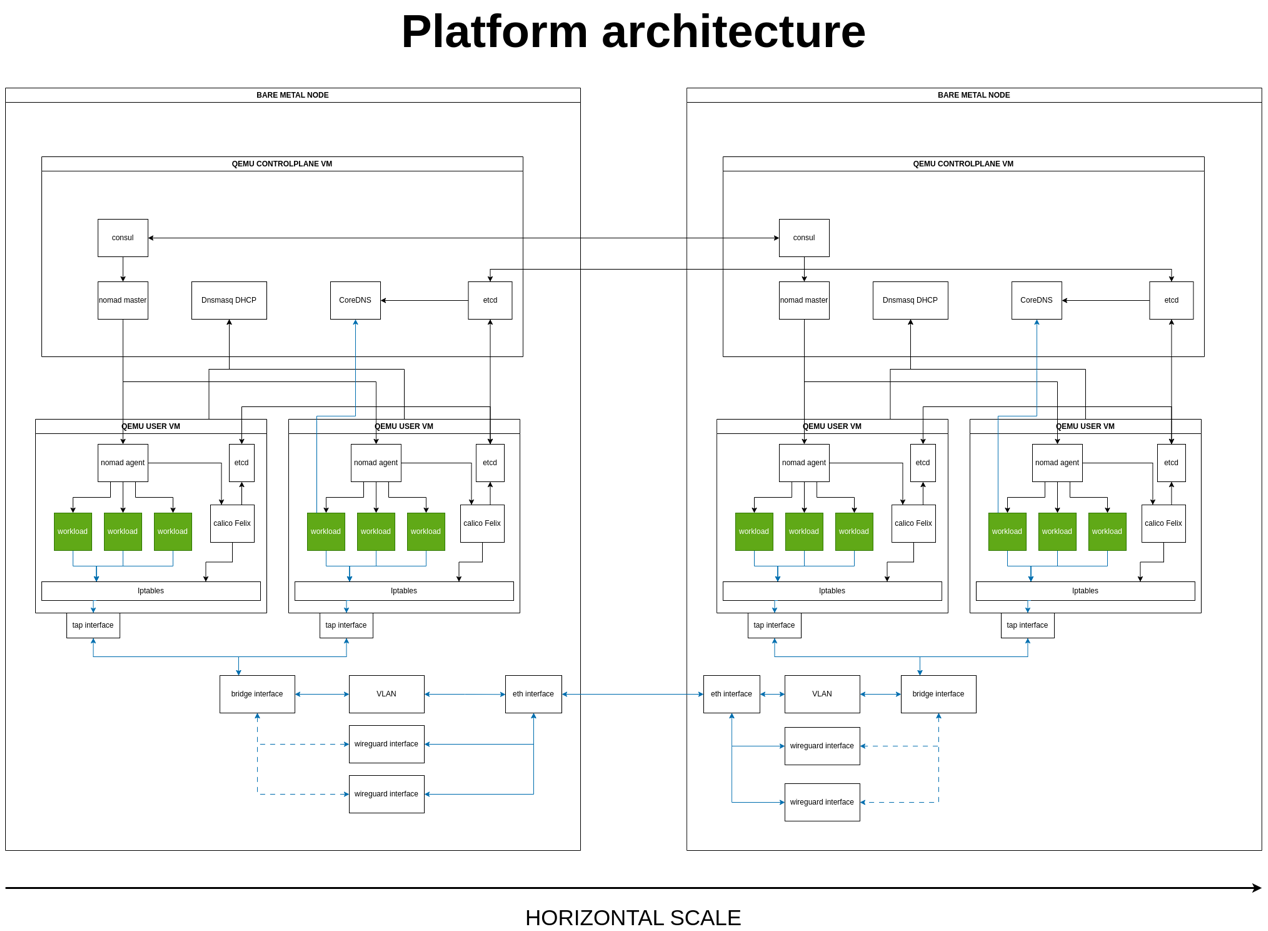
\includegraphics[width=0.8\textwidth]{media/ict/image18}
	\caption*{}
\end{figure}


{\bfseries Рис. 1 - Архитектура проекта BULT}

Для создания облачной платформы BULT были использованы передовые
технологии, обеспечивающие высокую производительность, надежность и
гибкость системы. Основные технологии включают контейнеризацию и
оркестрацию с использованием Docker и Nomad от HashiCorp {[}21{]}, что
позволяет изолировать приложения, обеспечивать их портативность и
эффективное использование ресурсов, а также динамически управлять
задачами, распределяя их между узлами кластера и обеспечивая высокую
доступность через интеграцию с Consul {[}22{]}. Управление данными
осуществляется через PostgreSQL {[}23{]}, мощную реляционную базу
данных, и JuiceFS, распределенное файловое хранилище, которые
обеспечивают высокую производительность, надежность и совместимость с
существующими приложениями {[}24{]}. Для безопасности используется
Wireguard для шифрования сетевого трафика и обеспечения безопасного
VPN-соединения, а также Let' s Encrypt для
автоматического получения и обновления SSL-сертификатов, что
обеспечивает шифрование данных между клиентом и сервером {[}25{]}.
Мониторинг и анализ системы реализуются с помощью Grafana и Loki
{[}26,27{]}, которые позволяют визуализировать метрики и логи,
обеспечивая оперативное обнаружение и устранение проблем. Принципы
DevOps и автоматизация процессов разработки, тестирования и
развертывания достигаются использованием CI/CD, что позволяет быстро и
безопасно внедрять изменения и новые функции, снижая количество ручной
работы и повышая качество и стабильность приложений. Эти технологии
создают прочную основу для дальнейшего развития и расширения
функциональности платформы BULT, отвечая современным требованиям и
вызовам в области облачных вычислений.

Функционал проекта BULT представляет собой облачную платформу,
включающую базовый набор функций для начальной операционной деятельности
и предоставления ключевых услуг пользователям, охватывающих широкий
спектр задач от базовой аутентификации до сложных операций с
Docker-образами и файлами. Платформа предлагает лендинг и панель
управления на трех языках (казахский, русский, английский), личный
кабинет для настройки учетных данных и управления проектами, создание,
удаление и редактирование проектов для гибкости и контроля разработки,
управление образами Docker с настройкой параметров, интерфейс для работы
с файлами и каталогами, API-слой для взаимодействия веб-приложения с
ядром, систему аутентификации и авторизации для безопасности данных,
авторизационного бота в Телеграм для управления доступом и запросов
поддержки, а также сервис для скачивания и управления Docker-образами.
Основные функции платформы обеспечивают гибкость и масштабируемость,
удобство управления через интуитивный интерфейс, эффективное управление
ресурсами, многоязыковую поддержку, безопасность и изоляцию данных, что
делает BULT конкурентоспособным решением на рынке облачных технологий,
предоставляя высокую производительность, надежность и удобство
эксплуатации веб-приложений.

\begin{figure}[H]
	\centering
	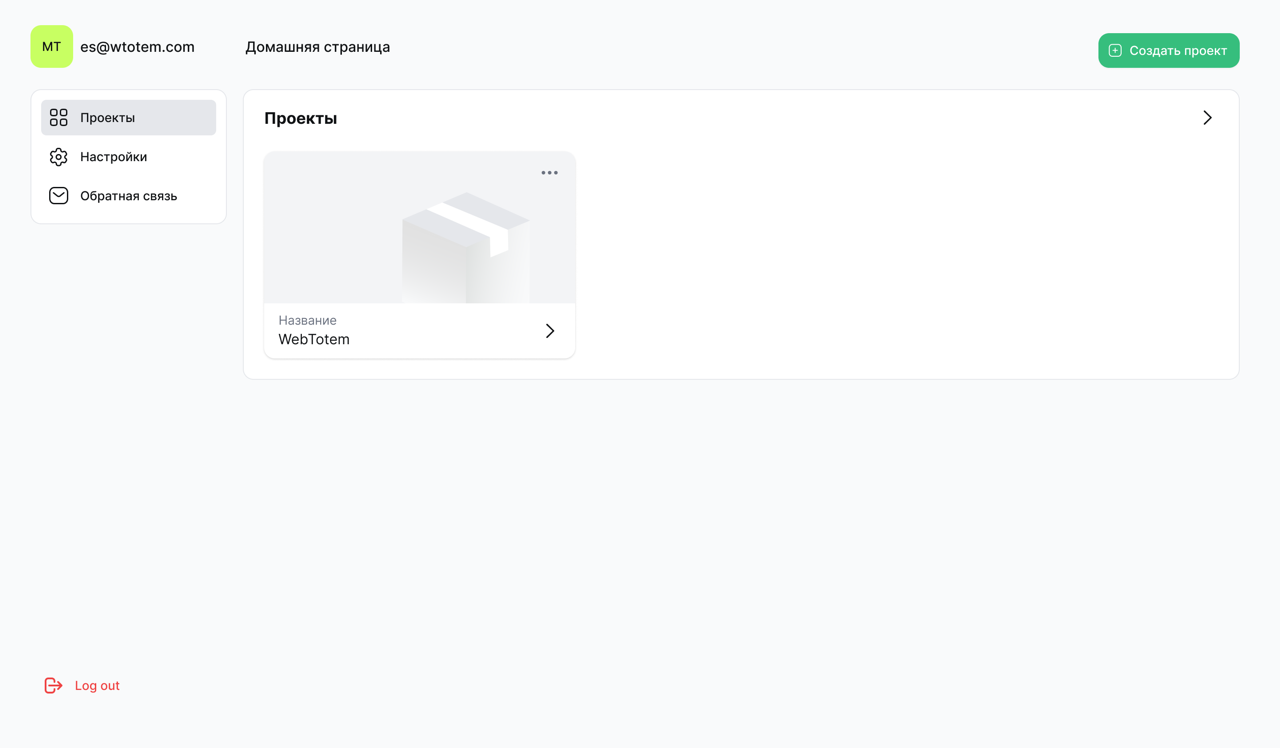
\includegraphics[width=0.8\textwidth]{media/ict/image19}
	\caption*{}
\end{figure}


{\bfseries Рис. 2 -- Панель управления}

\begin{figure}[H]
	\centering
	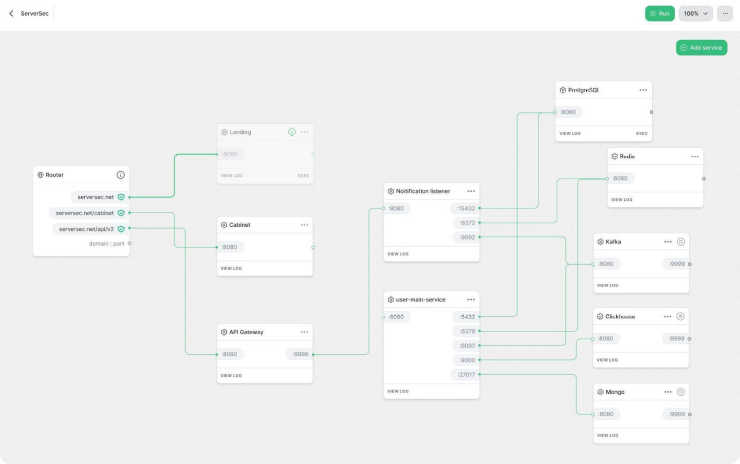
\includegraphics[width=0.8\textwidth]{media/ict/image20}
	\caption*{}
\end{figure}


{\bfseries Рис. 3 -- Запуск сервера}

\begin{figure}[H]
	\centering
	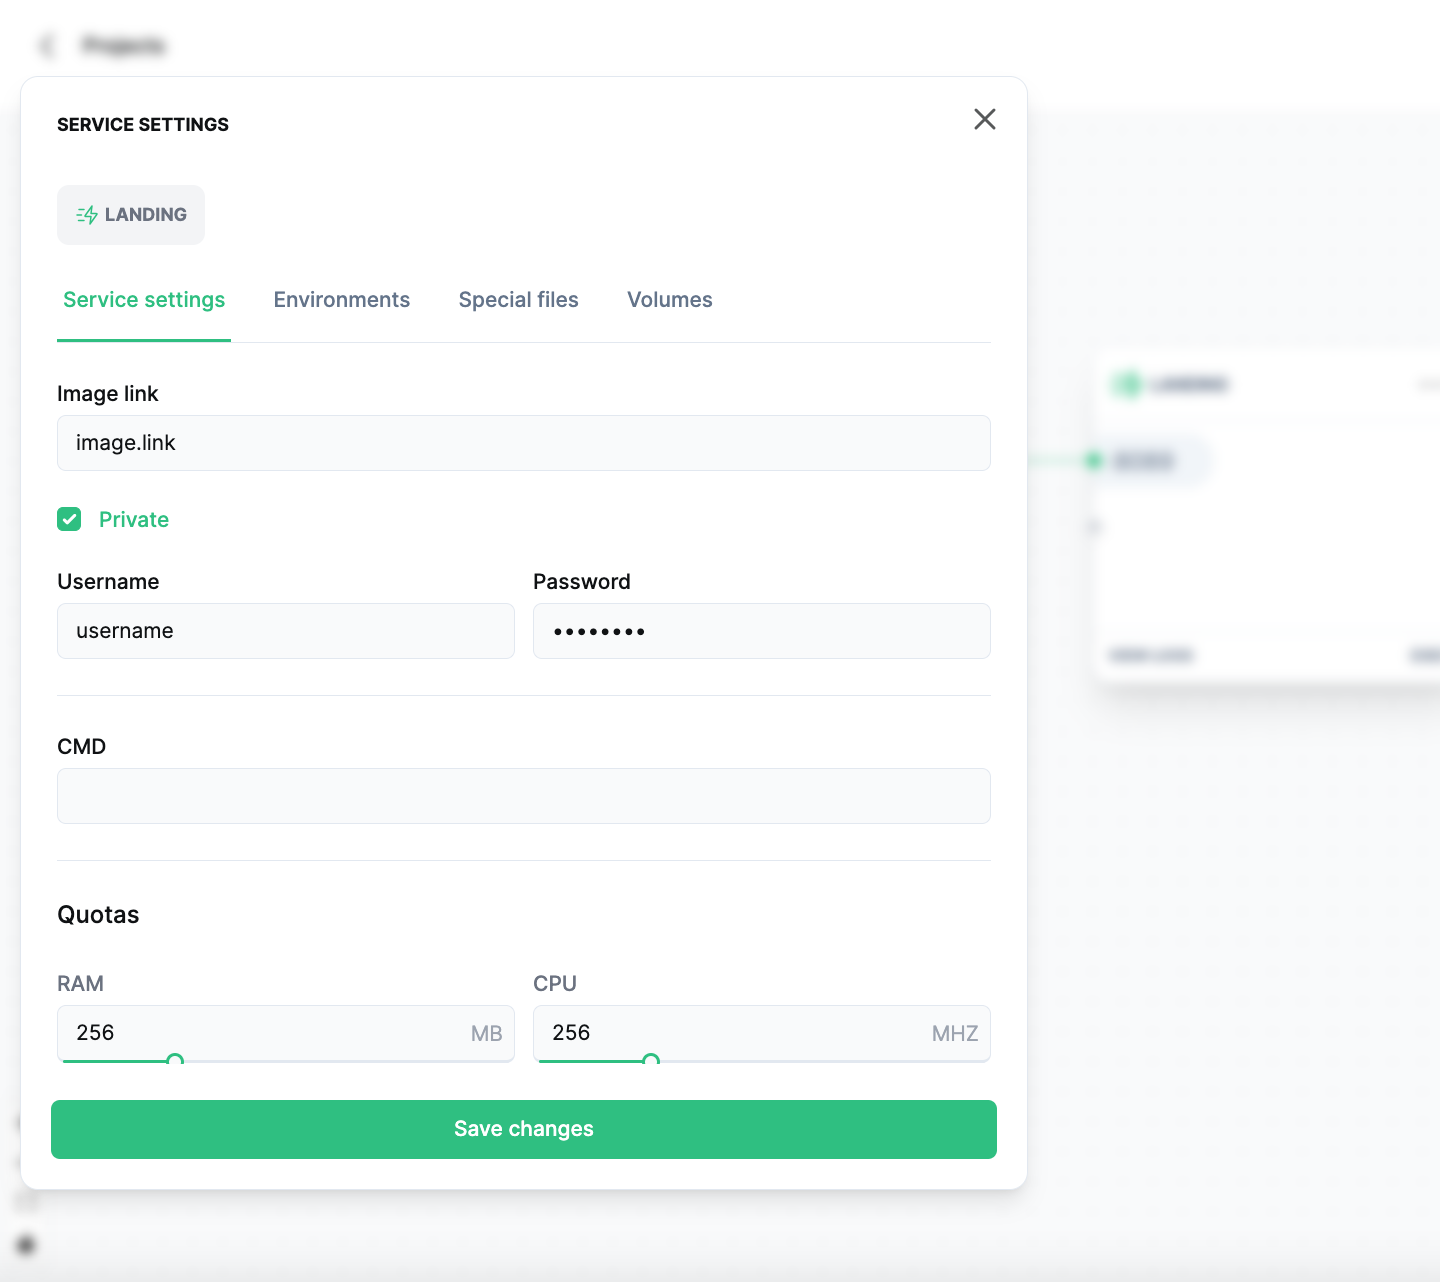
\includegraphics[width=0.8\textwidth]{media/ict/image21}
	\caption*{}
\end{figure}


{\bfseries Рис. 4 - Пример параметров для запуска сервиса с использованием
Docker}

На платформе BULT процесс разработки и оркестрации веб-приложений
включает несколько ключевых этапов. Сначала проводится определение
требований и проектирование архитектуры, что включает сбор требований,
установление целей проекта и разработку структуры системы. Далее
разрабатываются микросервисы, которые упаковываются в контейнеры с
использованием технологий, таких как Docker, для обеспечения изоляции и
портативности. Затем осуществляется оркестрация контейнеров с помощью
инструментов, например, Nomad от HashiCorp, для управления ресурсами и
масштабируемости. После интеграции всех компонентов и их тестирования в
единой среде, система развертывается в продуктивной среде с
использованием инструментов автоматического развертывания и управления,
таких как Kubernetes и Terraform. Мониторинг и анализ работы приложений
осуществляются с помощью инструментов, таких как Grafana и Loki. На
завершающем этапе производится поддержка и обновление системы для
обеспечения безопасности и функциональности, а также внедрение новых
функций и исправление ошибок в рамках процесса DevOps.

Платформа BULT была разработана с учетом современных требований к
разработке и управлению веб-приложениями, обеспечивая высокий уровень
производительности и надежности. Она предлагает гибкость и
масштабируемость благодаря модульной архитектуре и поддержке
микросервисов, что позволяет легко адаптировать разработки к
изменяющимся требованиям. Удобный интерфейс личного кабинета упрощает
управление учетными данными и проектами, а поддержка Docker-образов и
файловых операций способствует эффективному управлению ресурсами.
Встроенные системы аутентификации и авторизации гарантируют защиту
данных и контроль доступа, в то время как многоязычная поддержка делает
платформу доступной для пользователей из разных регионов. Результаты
тестирования продемонстрировали снижение времени отклика системы на 26\%
и увеличение устойчивости под нагрузкой на 18\% по сравнению с
традиционными решениями, подтверждая конкурентоспособность платформы
BULT на рынке облачных технологий и ее способность удовлетворять
современные требования к управлению веб-приложениями.

Платформа BULT продемонстрировала значительное превосходство по
сравнению с традиционными подходами благодаря применению
междисциплинарного подхода, который интегрирует знания и методы из
информатики, инженерных наук, информационной безопасности и менеджмента.
Это позволило значительно повысить надежность и производительность
платформы, улучшив качество веб-приложений. Инновационные архитектурные
решения, такие как микросервисная архитектура и контейнеризация,
обеспечили высокую гибкость и масштабируемость, в то время как передовые
методы шифрования и защиты сетевого трафика повысили уровень
безопасности данных. Внедрение практик DevOps автоматизировало процессы
разработки, тестирования и развертывания, что сократило время на
внедрение новых функций и повысило стабильность системы. Таким образом,
междисциплинарный подход делает платформу BULT уникальным и эффективным
решением для современных задач облачных систем, предлагая высокую
производительность, надежность и гибкость.

{\bfseries Выводы.}В данной статье мы представили облачную платформу BULT,
которая использует передовые технологии для разработки и оркестрации
веб-приложений. Платформа BULT обеспечивает гибкость, масштабируемость и
надежность, предлагая решения для современных вызовов в области облачных
технологий. Более детальную информацию о платформе, её архитектурных
решениях и преимуществах можно найти на официальном сайте BULT {[}28{]}.
Этот ресурс предоставляет доступ к дополнительным материалам, примерам
применения и информации о технологических особенностях платформы, что
позволяет глубже понять её возможности и преимущества в сравнении с
традиционными подходами.

\emph{{\bfseries Финансирование.} Инициативный научный проект выполнен за
счет собственных средств ТОО «Web Totem» на основании протокола №1 от
10.11.23г. Регистрационный номер № 0124РКИ0205, Инвентарный №
0224РКИ0306.}

{\bfseries Литература}

\begin{enumerate}
\def\labelenumi{\arabic{enumi}.}
\item
  Chen, L.~Microservices: Architecting for Continuous Delivery and
  DevOps~// 2018 IEEE International Conference on Software Architecture
  (ICSA). Seattle, WA, USA, 2018. - P. 39-397. DOI
  10.1109/ICSA.2018.00013
\item
  Mazzara, M., Dragoni, N., Bucchiarone, A., Giaretta, A., Larsen, S.
  T., Dustdar, S.~Microservices: Migration of a Mission Critical
  System~// IEEE Transactions on Services Computing. - 2021. - Vol.
  14(5)- P. 1464--1477. DOI 10.1109/TSC.2018.2889087
\item
  Singh, V., Peddoju, S. K.~Container-based Microservice Architecture
  for Cloud Applications~// 2017 International Conference on Computing,
  Communication and Automation (ICCCA). Greater Noida, India, 2017.- P.
  847 - 852. DOI 10.1109/CCAA.2017.8229914
\item
  Villamizar, M., Garcés, O., Castro, H., Verano, M., Salamanca, L.,
  Casallas, R., Gil, S.~Evaluating the Monolithic and the Microservice
  Architecture Pattern to Deploy Web Applications in the Cloud~// 2015
  10th Computing Colombian Conference (10CCC), 2015. -P. 583--590. DOI
  10.1109/ColumbianCC.2015.7333476
\item
  Barinov, A., Morozov, I., Melnikov, K. V., Rudenko, E.~Agentless
  Annotated Monitoring of User Behavioral Information in Container
  Infrastructures~// Journal of the Ural Federal District. Information
  Security. - 2023. -Vol. 23(1) DOI 10.14529/secur230102
\item
  Burns, B., Grant, B., Oppenheimer, D., Brewer, E., Wilkes, J.~Borg,
  Omega, and Kubernetes: Lessons Learned from Three Container-Management
  Systems over a Decade~// Queue. -2016. -Vol.14(1)- P. 70--93. DOI
  10.1145/2898442.2898444
\item
  Baškarada, S., Nguyen, V., Koronios, A.~Architecting Microservices:
  Practical Opportunities and Challenges~// Journal of Computer
  Information Systems. -2018. -Vol. 60(5) - P. 428--436. DOI
  10.1080/08874417.2018.1520056
\item
  Balalaie, A., Heydarnoori, A., Jamshidi, P.~Microservices Architecture
  Enables DevOps: Migration to a Cloud-Native Architecture~// IEEE
  Software. -2016. -Vol. 33(3)- P. 42--52. DOI 10.1109/MS.2016.64
\end{enumerate}

9. Omelchenko V., Rolik O. utomation of resource management in
information systems based on reactive vertical scaling// Адаптивні
Системи Автоматичного Управління. -2022. -Т.2(41)- С. 65 - 78. DOI
10.20535/1560-8956.41.2022.271344

10. Kusnandar, A.~Evaluation of Information System Security Using Fuzzy
FMEA Based on ISO/IEC 27001:2013 Framework to Improve Information
Security~//Journal of Business Information Systems. -2024.- Vol.14(2)-
P. 181- 190. DOI 10.21456/vol14iss2pp181-190

11. Cardarelli M., Iovino L., Francesco P. D., Salle A. D., Malavolta
I., Lago P. An extensible data-driven approach for evaluating the
quality of microservice architectures //~Proceedings of the 34th
ACM/SIGAPP Symposium on Applied Computing.- 2019.- P.1225-1234.

DOI
\href{https://doi.org/10.1145/3297280.3297400}{10.1145/3297280.3297400}

12.Femminella M., Palmucci M., Reali G., Rengo M. Attribute-based
management of secure Kubernetes cloud bursting //~IEEE Open Journal of
the Communications Society.-2024. -Vol. 5.- P. 1276 -1298. DOI
\href{https://doi.org/10.1109/ojcoms.2024.3367461}{10.1109/ojcoms.2024.3367461}

13.Desina G. C. Evaluating the impact of cloud-based microservices
architecture on application performance //arXiv preprint
arXiv:2305.15438. - 2023. DOI 10.48550/arXiv.2305.15438

14.Chen L., Xian M., \& Liu, J. Monitoring system of OpenStack cloud
platform based on Prometheus. 2020 International Conference on Computer
Vision, Image and Deep Learning (CVIDL). IEEE, pp. 206-209. DOI
10.1109/CVIDL51233.2020.0-100.

15.Wang M., Kulshrestha A., Wang L., Nordström L. Leveraging strategic
connection migration-powered traffic splitting for privacy
//~Proceedings on Privacy Enhancing Technologies.~-2022.-Vol.2022(3) -
P. 498 - 515.
DOI~\href{https://doi.org/10.56553/popets-2022-0083}{10.56553/popets-2022-0083}

16.Bezzateev S., Elina T. N., Mylnikov V. A. Modeling of selection
processes of cloud systems parameters providing their stability in
accordance with reliability and safety //~Scientific and Technical
Journal of Information Technologies, Mechanics and Optics.- 2018.-Vol.
18(4) - P. 654- 662. DOI
\href{https://doi.org/10.17586/2226-1494-2018-18-4-654-662}{10.17586/2226-1494-2018-18-4-654-662}

17.Hung M.-H., Lin Y.-C., Hsiao H.-C., Chen C.-C., Lai K.-C., Hsieh
Y.-M., Tieng H., Tsai T.-H., Huang H.-C., Yang H.-C., Cheng F.-T. A
novel implementation framework of digital twins for intelligent
manufacturing based on container technology and cloud manufacturing
services // IEEE Transactions on Automation Science and Engineering.-
2022.-Vol.19(3)- P.1614- 1630. DOI10.1109/TASE.2022.3143832

18.Kale S., et al. E-FireGuard: Empowering firefighters through
innovative E-commerce solutions //~Industrial Management
Advances.~-2024.-Vol.2(1)- P. 6375--6375.

DOI 10.59429/ima.v2i1.6375

19.Тарамов А.А., Черненькая Л.В. Описание инструментария для создания
современного CI/CD конвейера //Перспективы науки. -- 2020. - №12(135).-
С.74-77.

20.Безпятый М. В. Автоматизация и оптимизация процессов разработки и
развертывания в devops: применение современных методов и инструментов
//Инновации и инвестиции. -- 2023.- №. 7. - С. 458-464.

21.Брыжинская А.В., Чернова С.В. КРАТКО ПРО DOCKER // Теория и практика
современной науки. 2019. -№10 (52). - С. 33-35.

22. Munisso R., Chis A. E. Cloudmapper: A model-based framework for
portability of cloud applications consuming PaaS services//2017 25th
Euromicro International Conference on Parallel, Distributed and
Network-Based Processing (PDP).-2017.- P.132-139. DOI
10.1109/pdp.2017.94

23.PostgreSQL Documentation. URL:
\url{https://www.postgresql.org/docs/-}Дата обращения: 28.08.2024.

24.Lee J.,Kim M.,Shah S.A.R., Ahn S.U.,Yoon H.,Noh S.Y.Performance
evaluations of distributed file systems for scientific big data in FUSE
environment//Electronics.-2021.-Vol.10 (12) - P. 1471. DOI
~\href{https://doi.org/10.3390/electronics10121471}{10.3390/electronics10121471}

25.Grafana Documentation. URL: \url{https://grafana.com/docs/-} Дата
обращения: 28.08.2024.

26.Loki Documentation. URL: \url{https://grafana.com/oss/loki/} - Дата
обращения: 28.08.2024.

27.Тюменцев Д. В. Devops в эпоху облачных технологий: современные
практики и перспективы развития //Вестник науки.- 2023.-Т.2. -№. 8
(65).- С. 190-195.

28. BULT. {[}Электронный ресурс{]}. URL: \url{https://bult.pro-} Дата
обращения: 28.08.2024

{\bfseries References}

1.Chen, L.~Microservices: Architecting for Continuous Delivery and
DevOps~// 2018 IEEE International Conference on Software Architecture
(ICSA). Seattle, WA, USA, 2018. - P. 39-397.

DOI 10.1109/ICSA.2018.00013

2.Mazzara, M., Dragoni, N., Bucchiarone, A., Giaretta, A., Larsen, S.
T., Dustdar, S.~Microservices: Migration of a Mission Critical System~//
IEEE Transactions on Services Computing. - 2021. - Vol. 14(5)- P.
1464--1477. DOI 10.1109/TSC.2018.2889087

3.Singh, V., Peddoju, S. K.~Container-based Microservice Architecture
for Cloud Applications~// 2017 International Conference on Computing,
Communication and Automation (ICCCA). Greater Noida, India, 2017.- P.
847 - 852. DOI 10.1109/CCAA.2017.8229914

4.Villamizar, M., Garcés, O., Castro, H., Verano, M., Salamanca, L.,
Casallas, R., Gil, S.~Evaluating the Monolithic and the Microservice
Architecture Pattern to Deploy Web Applications in the Cloud~// 2015
10th Computing Colombian Conference (10CCC), 2015. -P. 583--590. DOI
10.1109/ColumbianCC.2015.7333476

5.Barinov, A., Morozov, I., Melnikov, K. V., Rudenko, E.~Agentless
Annotated Monitoring of User Behavioral Information in Container
Infrastructures~// Journal of the Ural Federal District. Information
Security. - 2023. -Vol. 23(1) DOI 10.14529/secur230102

6.Burns, B., Grant, B., Oppenheimer, D., Brewer, E., Wilkes, J.~Borg,
Omega, and Kubernetes: Lessons Learned from Three Container-Management
Systems over a Decade~// Queue. -2016. -Vol.14(1)- P. 70--93. DOI
10.1145/2898442.2898444

7.Baškarada, S., Nguyen, V., Koronios, A.~Architecting Microservices:
Practical Opportunities and Challenges~// Journal of Computer
Information Systems. -2018. -Vol. 60(5) - P. 428--436. DOI
10.1080/08874417.2018.1520056

8.Balalaie, A., Heydarnoori, A., Jamshidi, P.~Microservices Architecture
Enables DevOps: Migration to a Cloud-Native Architecture~// IEEE
Software. -2016. -Vol. 33(3)- P. 42--52. DOI 10.1109/MS.2016.64

9. Omelchenko V., Rolik O. utomation of resource management in
information systems based on reactive vertical scaling// Адаптивні
Системи Автоматичного Управління. -2022. -Т.2(41)- С. 65 - 78. DOI
10.20535/1560-8956.41.2022.271344

10. Kusnandar, A.~Evaluation of Information System Security Using Fuzzy
FMEA Based on ISO/IEC 27001:2013 Framework to Improve Information
Security~//Journal of Business Information Systems. -2024.- Vol.14(2)-
P. 181- 190. DOI 10.21456/vol14iss2pp181-190

11. Cardarelli M., Iovino L., Francesco P. D., Salle A. D., Malavolta
I., Lago P. An extensible data-driven approach for evaluating the
quality of microservice architectures //~Proceedings of the 34th
ACM/SIGAPP Symposium on Applied Computing.- 2019.- P.1225-1234.

DOI
\href{https://doi.org/10.1145/3297280.3297400}{10.1145/3297280.3297400}

12.Femminella M., Palmucci M., Reali G., Rengo M. Attribute-based
management of secure Kubernetes cloud bursting //~IEEE Open Journal of
the Communications Society.-2024. -Vol. 5.- P. 1276 -1298. DOI
\href{https://doi.org/10.1109/ojcoms.2024.3367461}{10.1109/ojcoms.2024.3367461}

13.Desina G. C. Evaluating the impact of cloud-based microservices
architecture on application performance //arXiv preprint
arXiv:2305.15438. - 2023. DOI 10.48550/arXiv.2305.15438

14.Chen L., Xian M., \& Liu, J. Monitoring system of OpenStack cloud
platform based on Prometheus. 2020 International Conference on Computer
Vision, Image and Deep Learning (CVIDL). IEEE, pp. 206-209. DOI
10.1109/CVIDL51233.2020.0-100.

15.Wang M., Kulshrestha A., Wang L., Nordström L. Leveraging strategic
connection migration-powered traffic splitting for privacy
//~Proceedings on Privacy Enhancing Technologies.~-2022.-Vol.2022(3) -
P. 498 - 515.
DOI~\href{https://doi.org/10.56553/popets-2022-0083}{10.56553/popets-2022-0083}

16.Bezzateev S., Elina T. N., Mylnikov V. A. Modeling of selection
processes of cloud systems parameters providing their stability in
accordance with reliability and safety //~Scientific and Technical
Journal of Information Technologies, Mechanics and Optics.- 2018.-Vol.
18(4) - P. 654- 662. DOI
\href{https://doi.org/10.17586/2226-1494-2018-18-4-654-662}{10.17586/2226-1494-2018-18-4-654-662}

17.Hung M.-H., Lin Y.-C., Hsiao H.-C., Chen C.-C., Lai K.-C., Hsieh
Y.-M., Tieng H., Tsai T.-H., Huang H.-C., Yang H.-C., Cheng F.-T. A
novel implementation framework of digital twins for intelligent
manufacturing based on container technology and cloud manufacturing
services // IEEE Transactions on Automation Science and Engineering.-
2022.-Vol.19(3)- P.1614- 1630. DOI10.1109/TASE.2022.3143832

18.Kale S., et al. E-FireGuard: Empowering firefighters through
innovative E-commerce solutions //~Industrial Management
Advances.~-2024.-Vol.2(1)- P. 6375--6375.

DOI 10.59429/ima.v2i1.6375

19.Taramov A.A., Chernen' kaja L.V. Opisanie
instrumentarija dlja sozdanija sovremennogo CI/CD konvejera
//Perspektivy nauki. -- 2020. - №12(135).- S.74-77.{[}in Russian{]}

20.Bezpjatyj M. V. Avtomatizacija i optimizacija processov razrabotki i
razvertyvanija v devops: primenenie sovremennyh metodov i instrumentov
//Innovacii i investicii. -- 2023.- №. 7. - S. 458-464.

21.Bryzhinskaja A.V., Chernova S.V. KRATKO PRO DOCKER // Teorija i
praktika sovremennoj

nauki. 2019. -№10 (52). - S. 33-35. {[}in Russian{]}

22. Munisso R., Chis A. E. Cloudmapper: A model-based framework for
portability of cloud applications consuming PaaS services//2017 25th
Euromicro International Conference on Parallel, Distributed and
Network-Based Processing (PDP).-2017.- P.132-139. DOI
10.1109/pdp.2017.94

23.PostgreSQL Documentation. URL:
\url{https://www.postgresql.org/docs/-}Дата обращения: 28.08.2024.

24.Lee J.,Kim M.,Shah S.A.R., Ahn S.U.,Yoon H.,Noh S.Y.Performance
evaluations of distributed file systems for scientific big data in FUSE
environment//Electronics.-2021.-Vol.10 (12) - P. 1471. DOI
~\href{https://doi.org/10.3390/electronics10121471}{10.3390/electronics10121471}

25.Grafana Documentation. URL: \url{https://grafana.com/docs/-} Data
obrashhenija: 28.08.2024.

26.Loki Documentation. URL: \url{https://grafana.com/oss/loki/} - Data
obrashhenija: 28.08.2024.

27.Tjumencev D. V. Devops v jepohu oblachnyh tehnologij: sovremennye
praktiki i perspektivy razvitija //Vestnik nauki.- 2023.-T.2. -№. 8
(65).- S. 190-195.{[}in Russian{]}

28. BULT. {[}Электронный ресурс{]}. URL: \url{https://bult.pro-} Data
obrashhenija: 28.08.2024.

\emph{{\bfseries Сведения об авторах}}

Шайханова А.К.- PhD, и.о. профессора кафедры информационной
безопасности, Евразийский национальный университет имени Л.Н.Гумилева,
Астана, Казахстан, e-mail:
\href{mailto:shaikhanova_ak@enu.kz}{\nolinkurl{shaikhanova\_ak@enu.kz}};

Бермухамбетов Ж.А.-Технический директор ТОО «WebTotem», e-mail:
\href{mailto:zb@wtotem.com}{\nolinkurl{zb@wtotem.com}};

Ким В.В.- Главный архитектор ТОО «WebTotem», Астана, Казахстан, e-mail:
\href{mailto:vk@wtotem.com}{\nolinkurl{vk@wtotem.com}};

Тлеубаева А.О.- докторант ТОО «Astana IT University», Астана, Казахстан,
e-mail:
\href{mailto:Arailym.tll@gmail.com}{\nolinkurl{Arailym.tll@gmail.com}}

\emph{{\bfseries Information about the authors}}

Shaikhanova A. K.-PhD, Acting Professor, Department of Information
Security, L.N. Gumilyov Eurasian National University, Astana,
Kazakhstan, e-mail:
\href{mailto:shaikhanova_ak@enu.kz}{\nolinkurl{shaikhanova\_ak@enu.kz}};

Bermukhambetov Zh.A.- Technical Director of LLP "WebTotem", Astana,
Kazakhstan, e-mail:
\href{mailto:zb@wtotem.com}{\nolinkurl{zb@wtotem.com}};

Kim V.V.- Chief Architect of LLP "WebTotem, Astana, Kazakhstan,
e-mail:\href{mailto:vk@wtotem.com}{\nolinkurl{vk@wtotem.com}};

Tleubayeva A.O. - PhD student of LLP «Astana IT University», Astana,
Kazakhstan, e-mail: Arailym.tll@gmail.com

{\bfseries ГРНТИ 28.23.15}

{\bfseries USING MACHINE LEARNING METHODS FOR AUTOMATIC TEXT PROCESSING OF
ABSTRACTS FROM SCIENTIFIC ARTICLES}

{\bfseries \textsuperscript{1}D. Kozybaev}
\begin{figure}[H]
	\centering
	
\includegraphics[width=0.8\textwidth]{media/ict/image1}
	\caption*{}
\end{figure}

\textsuperscript{2}G. Shangytbayeva}
\begin{figure}[H]
	\centering
	
\includegraphics[width=0.8\textwidth]{media/ict/image1}
	\caption*{}
\end{figure}

\textsuperscript{3}A. Zhakish}
\begin{figure}[H]
	\centering
	
\includegraphics[width=0.8\textwidth]{media/ict/image1}
	\caption*{}
\end{figure}

\textsuperscript{3}G. Muratova}
\begin{figure}[H]
	\centering
	
\includegraphics[width=0.8\textwidth]{media/ict/image1}
	\caption*{}
\end{figure}


{\bfseries \textsuperscript{4}B. Tassuov}
\begin{figure}[H]
	\centering
	
\includegraphics[width=0.8\textwidth]{media/ict/image1}
	\caption*{}
\end{figure}

Tanirbergenov}
\begin{figure}[H]
	\centering
	
\includegraphics[width=0.8\textwidth]{media/ict/image1}
	\caption*{}
\end{figure}


\emph{\textsuperscript{1}L.N. Gumilyov Eurasian National University,
Astana, Kazakhstan,}

\emph{\textsuperscript{2}K Zhubanov Aktobe Regional UniversityAktobe,
Kazakhstan,}

\emph{\textsuperscript{3} Korkyt Ata Kyzylorda University, Kyzylorda,
Kazakhstan,}

\emph{\textsuperscript{4}Taraz Regional University named after M.Kh.
Dulaty, Taraz, Kazakhstan}

{\bfseries \textsuperscript{\envelope }}Correspondent-author: t.adilbek@mail.ru

This paper examines the application of machine learning methods for
automatic text processing of abstracts from scientific articles. With
the increasing volume of scientific information, researchers are faced
with the problem of information overload, which makes it difficult to
find and analyze relevant materials. To solve this problem, we are
implementing machine learning algorithms such as the Support vector
Machine (SVM) method and word representation using Word2Vec, which
allows us to effectively classify annotations and extract key
information. In the process, we collect data from open databases.
Annotations go through preprocessing stages, including tokenization,
lemmatization, and deletion of stop words. Then we use Word2Vec to
convert annotation texts into vector representations, which serve as
input data for the SVM model. The effectiveness of the models is
evaluated using accuracy, completeness and F1-measure metrics. The
results show that the integration of SVM and Word2Vec significantly
improves the quality of annotation classification, which makes it
possible to speed up the process of searching for scientific
information. The work highlights the potential of using machine learning
methods to automate the processing of scientific texts and suggests
areas for further research, including the use of more complex models
such as transformers. This methodology can become the basis for the
development of effective tools that facilitate faster knowledge sharing
in the scientific community.

{\bfseries Keywords:} Machine learning, automatic text processing,
annotations, scientific articles, support vector machine (SVM),
Word2Vec.

{\bfseries ИСПОЛЬЗОВАНИЕ МЕТОДОВ МАШИННОГО ОБУЧЕНИЯ ДЛЯ АВТОМАТИЧЕСКОЙ
ОБРАБОТКИ ТЕКСТОВ АННОТАЦИЙ ИЗ НАУЧНЫХ СТАТЕЙ}

{\bfseries \textsuperscript{1}Д.Х. Козыбаев, \textsuperscript{2}Г.А.
Шангытбаева,} \textsuperscript{3}{\bfseries А.Н. Жәкіш,
\textsuperscript{3}Г.К. Муратова,}

{\bfseries \textsuperscript{4}Б. Тасуов, \textsuperscript{1}А.Ж.
Танирбергенов\textsuperscript{\envelope }}

\emph{\textsuperscript{1}Евразийский национальный университет имени
Л.Н.Гумилева, Астана, Казахстан,}

\emph{\textsuperscript{2}Актюбинский региональный университет
им.К.Жубанова, Актобе, Казахстан,}

\emph{\textsuperscript{3}Кызылординский университет им. Коркыт Ата,
Кызылорда, Казахстан,}

\emph{\textsuperscript{4}Таразский региональный университет им.М. Х.
Дулати, Тараз, Казахстан,}

\emph{e-mail: t.adilbek@mail.ru}

В данной работе рассматривается применение методов машинного обучения
для автоматической обработки текстов аннотаций из научных статей. С
увеличением объема научной информации исследователи сталкиваются с
проблемой информационной перегрузки, что затрудняет поиск и анализ
релевантных материалов. Для решения этой задачи мы внедряем алгоритмы
машинного обучения, такие как метод опорных векторов (SVM) и
представление слов с помощью Word2Vec, что позволяет эффективно
классифицировать аннотации и извлекать ключевую информацию. В процессе
работы мы осуществляем сбор данных из открытых баз данных. Аннотации
проходят этапы предобработки, включая токенизацию, лемматизацию и
удаление стоп-слов. Затем мы используем Word2Vec для преобразования
текстов аннотаций в векторные представления, которые служат входными
данными для модели SVM. Оценка эффективности моделей проводится с
использованием метрик точности, полноты и F1-меры. Результаты
показывают, что интеграция SVM и Word2Vec значительно улучшает качество
классификации аннотаций, что позволяет ускорить процесс поиска научной
информации. Работа подчеркивает потенциал использования методов
машинного обучения для автоматизации обработки научных текстов и
предлагает направления для дальнейших исследований, включая применение
более сложных моделей, таких как трансформеры. Данная методология может
стать основой для разработки эффективных инструментов, способствующих
более быстрому обмену знаниями в научном сообществе.

{\bfseries Ключевые слова:} Машинное обучение, автоматическая обработка
текста, аннотации, научные статьи, опорный вектор машине (SVM),
Word2Vec.

{\bfseries ҒЫЛЫМИ МАҚАЛАЛАРДАН АВТОМАТТЫ ТҮРДЕ АННОТАЦИЯ МӘТІНДЕРІН ӨҢДЕУ
ҮШІН МАШИНАЛЫҚ ОҚЫТУ ӘДІСТЕРІН ҚОЛДАНУ}

{\bfseries \textsuperscript{1}Д.Х. Козыбаев, \textsuperscript{2}Г.А.
Шангытбаева,} \textsuperscript{3}{\bfseries А.Н. Жәкіш,
\textsuperscript{3}Г.К. Муратова, \textsuperscript{4}Б. Тасуов}

{\bfseries \textsuperscript{1}А.Ж. Танирбергенов\textsuperscript{\envelope }}

\emph{\textsuperscript{1}Л.Н.Гумилев атындағы Еуразия ұлттық
университеті, Астана қ., Қазақстан,}

\emph{\textsuperscript{2}Қ.Жұбанов ат.Ақтөбе өңірлік университеті,
Ақтөбе қ., Қазақстан,}

\emph{\textsuperscript{3}Қорқыт Ата атындағы Қызылорда университеті,
Қызылорда қ., Қазақстан,}

\emph{\textsuperscript{4}М.Х.Дулати атындағы Тараз өңірлік университеті,
Тараз қ., Қазақстан,}

\emph{e-mail: t.adilbek@mail.ru}

Бұл жұмыста ғылыми мақалалардағы аннотация мәтіндерін автоматты түрде
өңдеу үшін машиналық оқыту әдістерін қолдану қарастырылады. Ғылыми
ақпараттың ұлғаюымен зерттеушілер ақпараттың шамадан тыс жүктелу
проблемасына тап болады, бұл тиісті материалдарды табу мен талдауды
қиындатады. Бұл мәселені шешу үшін біз аннотацияларды тиімді жіктеуге
және негізгі ақпаратты алуға мүмкіндік беретін Word2Vec көмегімен
анықтамалық векторлық әдіс (SVM) және сөздерді ұсыну сияқты Машиналық
оқыту алгоритмдерін енгіземіз. Жұмыс барысында біз ашық мәліметтер
базасынан мәліметтер жинаймыз. Аннотациялар токенизация, лемматизация
және тоқтату сөздерін жоюды қоса алғанда, алдын ала өңдеу кезеңдерінен
өтеді. Содан кейін біз Аннотация мәтіндерін SVM моделіне кіріс ретінде
қызмет ететін векторлық көріністерге түрлендіру үшін Word2Vec
қолданамыз. Модельдердің тиімділігін бағалау дәлдік, толықтық және F1
өлшемдерін қолдану арқылы жүзеге асырылады. Нәтижелер SVM және Word2Vec
интеграциясы Аннотация классификациясының сапасын айтарлықтай
жақсартады, бұл ғылыми ақпаратты іздеу процесін жылдамдатуға мүмкіндік
береді. Жұмыс ғылыми мәтіндерді өңдеуді автоматтандыру үшін машиналық
оқыту әдістерін қолдану әлеуетіне баса назар аударады және одан әрі
зерттеуге, соның ішінде трансформаторлар сияқты күрделі модельдерді
қолдануға бағыттар ұсынады. Бұл әдістеме ғылыми қоғамдастықта біліммен
жылдам алмасуға ықпал ететін тиімді құралдарды әзірлеуге негіз бола
алады.

{\bfseries Түйін сөздер:} Машиналық оқыту, мәтінді автоматты өңдеу,
аннотациялар, ғылыми мақалалар, анықтамалық векторлық әдіс (SVM),
Word2Vec.

{\bfseries Introduction.} The modern scientific community produces a huge
number of publications, and annotations to them play a key role in
providing quick access to the main research results. Annotations are
short summaries that outline the goals, methods, and main conclusions of
the work. However, with the increasing volume of information, the
processing and analysis of these annotations are becoming more and more
complex tasks. In this regard, machine learning and natural language
processing (NLP) methods are becoming necessary tools for automating
word processing processes {[}1{]}.

One of the main problems is information overload. Scientists and
researchers often face the need to browse through thousands of abstracts
to find relevant articles for their work. For example, millions of
articles are published annually in the field of biomedical research, and
manual analysis of all annotations becomes almost impossible. As a
result, researchers may miss important discoveries or relevant research,
which slows down progress in science.

Another major problem is the variety of annotation formats and writing
styles. Different journals and authors may use different approaches to
writing annotations, which makes it difficult to automatically process
and analyze the text. For example, some annotations may be very brief
and concise, while others may contain many technical terms and complex
sentences. This diversity requires the development of adaptive methods
that can effectively work with different styles and formats {[}2{]}.

In addition, there is a problem of ambiguity and ambiguity of terms. In
the scientific literature, the same terms can be used in different
contexts, which can lead to incorrect interpretation of information. For
example, the term "parameter" can refer to both a mathematical concept
and a biological aspect, depending on the context. This makes the task
of extracting information even more difficult, requiring algorithms to
understand the content of the text in depth {[}3{]}.

It is also worth noting the problem of incompleteness and insufficient
information content of annotations. Some annotations may not contain
enough information to understand the essence of the study, which makes
it difficult to use them for further analysis. For example, if the
abstract does not indicate key methods or results, this may lead to a
misunderstanding of the work and its significance

In recent years, there has been a sharp increase in the volume of
scientific information, which creates significant difficulties in the
process of its analysis and synthesis. A huge number of articles in
various fields of knowledge are published every day, and researchers
need to quickly navigate this flow of information, select the most
relevant materials and extract valuable data. In such conditions,
automation of text information processing becomes particularly relevant,
which can largely be achieved using machine learning methods.

Machine learning, being one of the most dynamically developing areas of
artificial intelligence, provides powerful tools for text analysis. It
allows not only to process large amounts of data, but also to identify
hidden patterns, classify, cluster and extract information. In
particular, machine learning methods can be effectively applied to the
automatic processing of abstracts of scientific articles, which
significantly speeds up the process of information retrieval and
analysis {[}4{]}.

This work is aimed at studying and applying modern machine learning
methods to automate the processing of annotations from scientific
articles {[}5{]}. The main object of research is annotations, which are
short summaries of the content of articles and contain key points and
research results. The availability of qualitatively processed
annotations can significantly increase the effectiveness of both
scientific work and the practical application of the acquired knowledge.

An important part of this study is the analysis of existing machine
learning algorithms such as Naive Bayes, Support Vector Machines and
neural networks. Each of these approaches has its advantages and
disadvantages, which will be considered in the context of annotation
processing. For example, Naive Bayes and SVM show high efficiency in
classification tasks, but neural networks, due to their ability to learn
from large amounts of data, can provide a deeper understanding of the
context and meanings of texts.

{\bfseries Methods and materials.} In this paper, I propose to use the
support Vector Machine (SVM) and Word2Vec methods as a hybrid model to
automatically extract annotations from scientific articles. SVM is a
powerful machine learning model, and Word2Vec is a neural network method
for determining the semantic relationships of words in texts. By
combining the two methods, we aim to achieve effective and accurate
results. Support Vector Machine (SVM) -- used for data classification in
high-dimensional space. This model identifies crucial hyperparallel when
classifying objects, which makes it possible to distinguish them to the
maximum. One of the biggest advantages of SVM is its efficiency and
accuracy, especially for classification work. The main advantages of
SVM:

- SVM provides effective results in the processing of complex and
nonlinear data.

- SVM produces new data in a good public way, which allows the model to
work effectively even in the test set.

- SVM models allow you to select parameters using kernel functions,
which helps you build an optimal model depending on the complexity of
the data.

Another feature of the SVM model is that it can be used with efficiency
when working with extremely large and complex data sets {[}6{]}. In
addition, the choice of different kernel functions for SVM ensures that
the model adapts according to the data description. Word2Vec is a neural
network model used to determine the semantic relationships of words in
texts. It provides the transfer of words in context to a vector form,
thus allowing the relationships between words to be expressed in
mathematical form. The Word2Vec model helps you learn from large volumes
of texts and understand the semantic values of words.

The main advantages of Word2Vec:

- Word2Vec allows you to understand the meaning of words by reading them
in their context, that is, the connections between words.

- Word2Vec allows you to reduce the amount of data by speeding up the
vectorization process, thus making the model learning process more
efficient.

- Word2Vec is used in various natural language processing tasks,
including text classification, text generation, annotation generation,
etc.

The advantage of Word2Vec is that it can effectively define the semantic
relationships of words in large volumes of text. This process allows you
to effectively understand the semantic relationships of words in the
context of scientific texts {[}7{]}. By combining the SVM and Word2Vec
models, we can take advantage of the two models. The powerful
classification capability of SVM and Word2Vec' s ability
to detect semantic connections provide high accuracy and efficiency in
automatically extracting annotations from scientific articles.
Advantages of the hybrid model:

- The combination of SVM and Word2Vec allows you to improve the quality
of annotations, because SVM is distinguished by its ability to classify,
and Word2Vec is used to understand the meanings of words.

- Comparing the results obtained to assess the effectiveness between the
models, allows a deeper analysis of the research topic.

- The hybrid model allows you to increase efficiency and performance by
optimizing parameters. The results of our model are not limited to a
combination of SVM and Word2Vec, but allow us to determine their
effectiveness by comparing them with additional alternative models.

This paper examines the application of machine learning methods for
automatic text processing of abstracts from scientific articles. With
the increasing volume of scientific information, researchers face the
problem of information overload, which makes it difficult to find and
analyze relevant materials. To address this issue, we implement machine
learning algorithms such as the Support Vector Machine (SVM) method and
word representation using Word2Vec, enabling effective annotation
classification and key information extraction.

We use random Forest, Naive Bayes, and NLTK-based models as these
alternative models. The results obtained suggest new approaches that
allow you to improve the accuracy and quality of annotations. Thus, our
research is aimed at improving the process of producing automated
annotations, which contributes to the effective processing of scientific
papers and literature.

In our study, in addition to the SVM and Word2Vec hybrid model for
producing automated annotations, I will also consider several
alternative models. These models help improve the accuracy of results
using various machine learning techniques. The theoretical foundations
and advantages of each model will be discussed below.

Random Forest is an ensemble machine learning model that uses decision
trees. It works by creating multiple decision trees (branches) and
combining their results. When Random Forest classifies data, each tree
gives its own forecast, and the final result is based on the voting
result of the forecasts of all trees.

Advantages:

- Random Forest effectively processes complex data, thanks to the
principle of majority voting.

- Reduces the potential defects of the model due to obtaining results
among many trees.

- Random Forest shows good results in working with large data sets.

NLTK (Natural Language Toolkit) is an advanced Python library for
editing natural languages. This tool provides various algorithms for
text analysis, classification, annotation and many other tasks. Using
the NLTK functionality, you can simplify the process of automatically
extracting annotations from texts.

Advantages:

- NLTK provides various functions for text processing, such as word
splitting, stemming, and lemmatization.

− Allows the user to simplify the settings when working with text data.

- NLTK is useful in scientific research and for testing new algorithms.

In our study, compared to the SVM + Word2Vec model, it is also important
to evaluate the results of the alternative models mentioned above. This
comparison provides new approaches that allow you to increase the
efficiency of publishing annotations.

Consideration of alternative models will allow us to further improve the
process of producing automated annotations, evaluate the results of
various approaches, and develop new solutions and proposals based on
them {[}8{]}.

Thus, together with the SVM + Word2Vec model, alternative models are
important elements that contribute to improving the process of producing
automated annotations.

It is very important to compare the results of the SVM + Word2Vec model
and alternative models (Random Forest and NLTK), which were used to
produce automated annotations in the study. The main purpose of the
comparison is to show the advantages of my main model and determine
under what conditions alternative models can be effective. The results
of the comparison of models can be seen in Figure-1 the accuracy and the
F1 score arrow.

\begin{figure}[H]
	\centering
	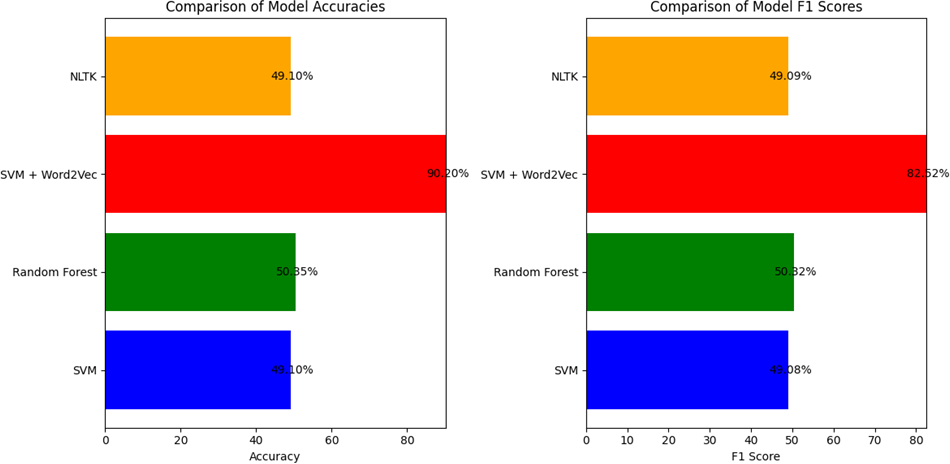
\includegraphics[width=0.8\textwidth]{media/ict/image22}
	\caption*{}
\end{figure}


{\bfseries Fig.1 - F1 score indicators with accuracy of models}

The results of the SVM + Word2Vec model are very high, as its accuracy
is 90.20\%, and the F1 Score is 82.52\%. This result determines the
strength and efficiency of the combination of SVM and Word2Vec models.
The SVM algorithm is effective for classifying text data, while Word2Vec
helps understand conceptuality and semantic relationships. As a result,
the SVM + Word2Vec model allows you to make high-precision predictions
for annotating texts.

In contrast, the Random Forest model showed 50.35\% accuracy and 50.32\%
F1 Score. The results of this model, of course, are much lower than the
level of the SVM + Word2Vec model. Random Forest uses many decision
trees as an ensemble model, however, it may not understand the semantic
structure of textual data well. The complexity and variation of textual
information is a challenge for the Random Forest model, so its
effectiveness is low.

The NLTK model also shows weaker results compared to the SVM + Word2Vec
model with an accuracy of 49.10\% and an F1 Score of 49.09\%. NLTK is a
tool for editing natural languages, but it is difficult to limit it to
its own algorithms for producing automatic annotations. As a result, the
NLTK model cannot provide the accuracy necessary for the main task,
which is associated with the complexity of textual data.

The SVM + Word2Vec model allows you to understand texts in depth,
because Word2Vec understands the semantic relationships of words using
contextual vectors. This model best defines how words in a text are
related to each other. As a result, SVM + Word2Vec has the highest
efficiency and accuracy when producing annotations.

The advantage of the Random Forest model is that it works on the
principle of majority voting. It combines many decision trees, but does
not take into account the natural features of textual data {[}9{]}. The
low performance of the model is due to the limitations of its text
comprehension mechanism, as variations and contexts of text data pose a
challenge for Random Forest.

The NLTK model provides a wide range of natural language processing
tools, but the difficulties in using these tools to produce automated
annotations indicate its limited effectiveness. NLTK mechanisms require
additional processing steps when working with text data, which reduces
the performance of the model.

The SVM + Word2Vec model shows high results with its characteristic
features and is therefore the main choice in the production of automated
annotations. The high accuracy and F1 Score indicators indicate the
effective solutions proposed by the model in the annotation of texts.

In comparison, the Random Forest and NLTK models experience difficulties
when working with text data (Figure - 2, 3). The results do not reach
the level of the SVM + Word2Vec model, which indicates their limitations
in processing the complexity of text data (Figure -4). In the task of
automated annotation of texts, the success of the SVM + Word2Vec model
lies in its good understanding of contextual information.

\begin{figure}[H]
	\centering
	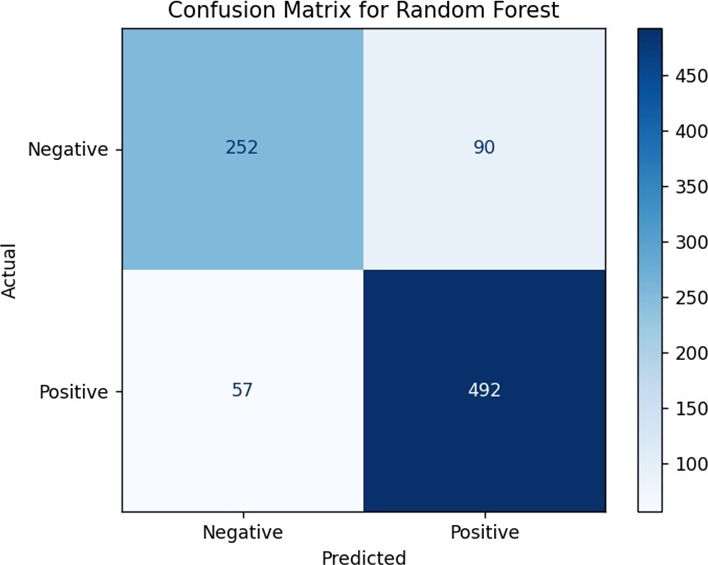
\includegraphics[width=0.8\textwidth]{media/ict/image23}
	\caption*{}
\end{figure}


{\bfseries Fig. 2 - Random Forest models of the Confusion Matrix (shatasu
matrixes) graphics}

\begin{figure}[H]
	\centering
	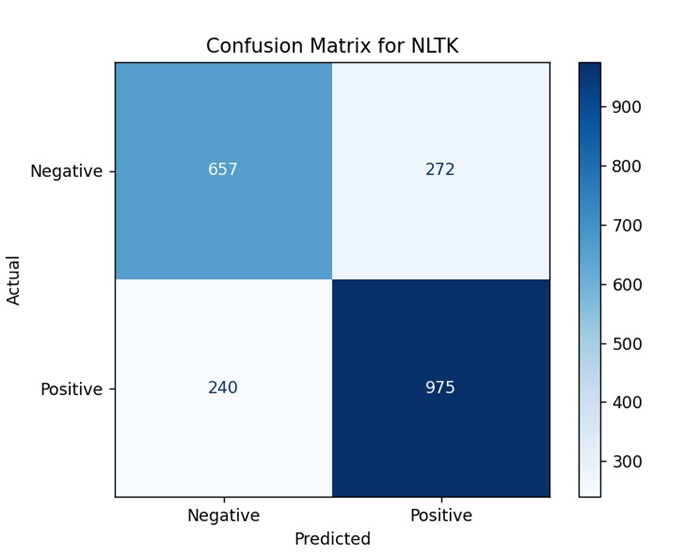
\includegraphics[width=0.8\textwidth]{media/ict/image24}
	\caption*{}
\end{figure}


{\bfseries Fig.3 - Confusion Matrix (confusion matrix) graph of the NLTK
model}

\begin{figure}[H]
	\centering
	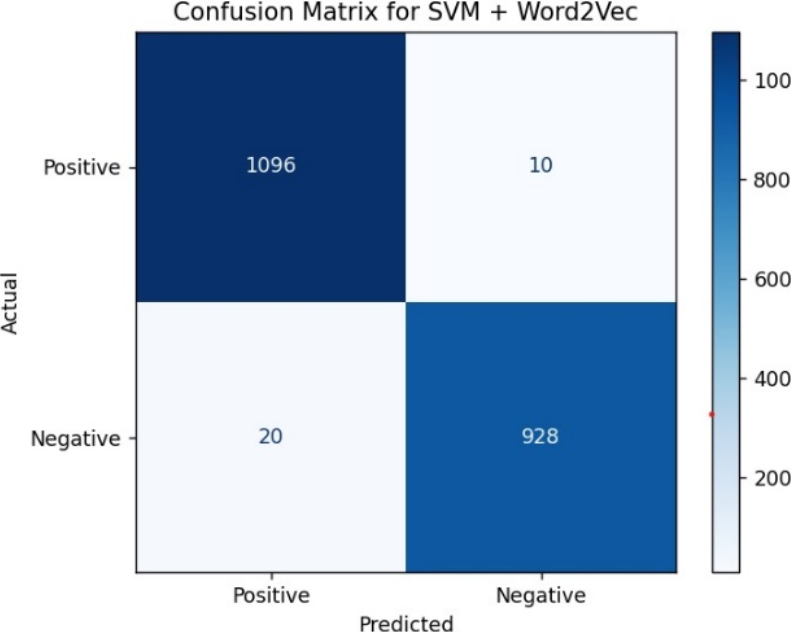
\includegraphics[width=0.8\textwidth]{media/ict/image25}
	\caption*{}
\end{figure}


{\bfseries Fig.4 - Graph of the Confusion Matrix of the hybrid model}

These images depict the results of three different models: Random
Forest, NLTK, and SVM + Word2Vec. How correctly each model predicts in
comparison with real data is shown using the Confusion Matrix (confusion
matrix). Random Forest model (Figure 2): The Random Forest model showed
252 correct and 90 incorrect results in predicting real negatives. For
real positives, 492 correct and 57 incorrect predictions were made. It
is obvious that the amount of incorrect prediction of this model is
quite high.

The classification accuracy of this model is at an average level, as the
error rate is still high. NLTK model (Figure 3): the result of the NLTK
model is also shown. In this model, when predicting real negatives, 657
correct and 272 incorrect results were obtained, and when predicting
real positives, 975 correct and 240 incorrect results were made. The
NLTK model has a higher error rate than the Random Forest model.

This model makes significant errors not only in predicting the
positives, but also in predicting the negatives, so its overall result
can be judged as inefficient. SVM + Word2Vec model (Figure 4): the SVM +
Word2Vec model showed significantly higher results. In predicting real
positives, 1096 correct and only 10 incorrect results were obtained, and
928 correct and 20 incorrect results were made for real negatives.

A detailed analysis of the model' s errors revealed that
the majority of false positives occurred in abstracts containing
ambiguous terms (e.g., "parameter" in both mathematical and biological
contexts). False negatives were more common in abstracts with incomplete
or overly concise information. To address these issues, future work
could incorporate domain-specific ontologies to disambiguate terms and
improve the model' s ability to handle incomplete
annotations.

These indicators are much better compared to other models, because the
number of errors is very small. The SVM + Word2Vec model classifies data
very efficiently and accurately, making it the most reliable and
high-performance model. In conclusion, when comparing these three
models, the SVM + Word2Vec model is the clear leader. It achieves more
realistic results than other models and has a very low error rate.
Therefore, as the most effective solution to the problem of automatic
classification of texts, it is proposed to use the SVM + Word2Vec model.
In general, the SVM + Word2Vec model is an effective solution for text
annotation, and alternative models, especially Random Forest and NLTK,
show their limitations when working with text data {[}10{]}. This
comparison allows you to evaluate machine learning approaches to produce
automated annotations, as well as provide the necessary information for
future research and model improvements. Our study confirms that the
relatively high performance of the SVM + Word2Vec model is the most
effective solution for automated annotation. Comparison of its results
with Random Forest and NLTK models determines the effectiveness of the
main models in processing text data.

{\bfseries Results and discussion.} Architecture of the model used. In our
today' s study, for the purpose of automatic text
annotation, the SVM + Word2Vec hybrid model was used to achieve the main
goal in my thesis topic. Now I will consider how in the architecture of
this gmbrid model it is possible to process texts more efficiently and
automatically extract the necessary information. The architecture of the
model can be seen in Figure 5 below.

\begin{figure}[H]
	\centering
	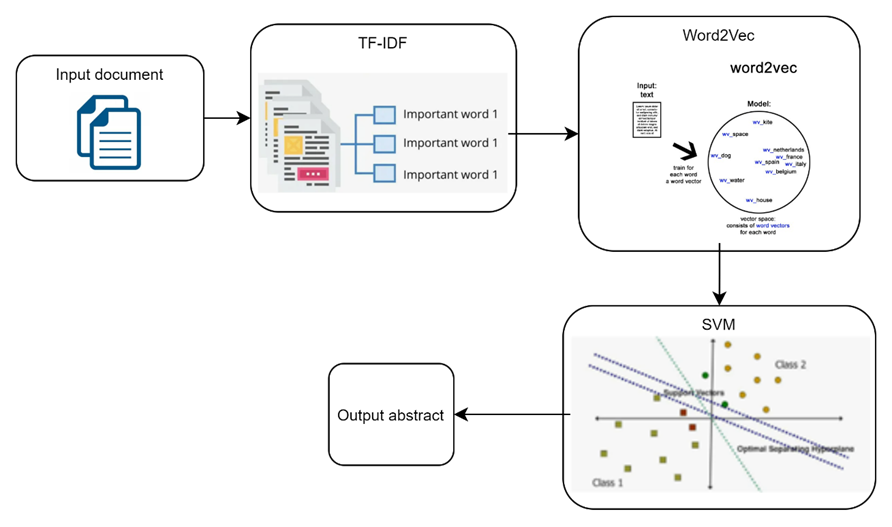
\includegraphics[width=0.8\textwidth]{media/ict/image26}
	\caption*{}
\end{figure}


{\bfseries Fig. 5- SVM + Word2Vec hybrid model architecture}

The process starts with an input document. At this stage, a scientific
article or other textual information obtained as an object of study is
loaded. The input text should correspond to the research topic, since
its content directly affects the quality of the annotation.

At the next stage, the TF-IDF (Term Frequency-Inverse Document
Frequency) algorithm is used. TF-IDF helps determine the importance of
each word in the text. The algorithm is used to calculate the frequency
(TF) of each word and how rare it is in the entire data set (IDF). As a
result, only the most important words are selected and their weight is
set. This stage is designed to identify the most important elements of
the text, because when compiling an annotation, it is advisable to use
only the main information.

After TF-IDF, the Word2Vec model is used. Word2Vec translates words in
text into vector space, which allows you to study the relationship
between the meaning and context of words. The model assigns a vector to
each word and contributes to understanding the semantic relationships of
words. As a result, each word is displayed in a vector form, which is
effective for embedding in a machine learning model.

Finally, the SVM (support Vector Machine) algorithm is implemented. SVM
is a classification algorithm that allows you to divide data (for
example, annotated texts) into two or more classes. SVM stands out for
its efficiency and scalability, which makes it suitable for use in large
data sets. Based on the vector forms of words, SVM performs data
separation, thus, the process of understanding and annotating important
information is carried out.

The next step is to get the output abstract. All components of the model
work together, as a result of which a brief annotation of the text is
automatically compiled. This annotation covers the content and important
aspects of the incoming document.

Also, as the results of the model showed during the comparison, the SVM
+ Word2Vec model achieved high efficiency. For example, the accuracy of
SVM was 49.10\%, while the accuracy of Random Forest was 50.35\%. And
the combination of SVM + Word2Vec reached an accuracy of 90.20\%, and
the F1 reading was 82.52\%. These results show that the SVM + Word2Vec
model is significantly ahead of other alternative models.

While the proposed SVM + Word2Vec model demonstrates strong performance,
transformer-based models such as BERT and GPT have shown remarkable
results in text classification tasks. However, the computational cost of
training and deploying transformer models is significantly higher,
making the SVM + Word2Vec model a more practical choice for
resource-constrained environments. Future work could explore hybrid
approaches that combine the efficiency of SVM with the contextual
understanding of transformers.

The efficiency and high results of the model will serve as the basis for
further study of text processing methods in the future. The SVM +
Word2Vec model can be widely used in informatization and annotation
systems, which increases automation and efficiency.

The SVM + Word2Vec model is the best solution for automatic text
annotation. The effectiveness and high results of the model are the main
achievement of my research. The annotations obtained as a result of this
work make it possible to understand and evaluate scientific articles
faster, thereby helping researchers to extract useful information more
efficiently.

{\bfseries Conclusion.} The proposed SVM + Word2Vec model offers a
computationally efficient and effective solution for automatic text
annotation of scientific articles. However, future research could
explore hybrid models that combine the strengths of SVM with
transformer-based approaches, such as BERT or RoBERTa. Additionally, the
use of domain-specific embeddings could further enhance the
model' s ability to capture nuanced semantic
relationships. Finally, extending the model to handle multi-lingual
scientific texts would broaden its applicability and impact in the
global scientific community.

The main goal of our research was to use word processing methods to
automatically extract annotations from scientific articles. In the
course of the study, the SVM + Word2Vec hybrid model was used, the
effectiveness and accuracy of this model made it possible to consider
the topic of the study in depth. As a result, the SVM + Word2Vec model
showed significant advantages over alternative models, reaching 90.20\%
accuracy and 82.52\% F1.

In the course of the study, the combination of the TF-IDF algorithm and
the Word2Vec model made it possible to identify the most important words
in the text and translate them into vector space. The SVM algorithm
provided an effective division of texts into two or more classes,
thereby simplifying the process of producing automated annotations.

Alternative models, such as NLTK and Random Forest, have shown much
lower accuracy results compared to the SVM + Word2Vec model, which
confirms the priority of SVM + Word2Vec in automatic annotation systems.
The NLTK model had an accuracy of 49.10\%, and the Random Forest model
had an accuracy of 50.35\%. These results showed that the SVM + Word2Vec
model plays a leading role in the efficient processing and annotation of
scientific texts.

The results of the study make it possible to deeply understand the
content of the text, automatically extract information and effectively
evaluate scientific work. This model may be widely used in
informatization and annotation systems in the future. In addition, the
combination of SVM + Word2Vec will guide future research in the field of
automatic text processing.

In conclusion, the SVM + Word2Vec model is the most effective solution
for automatically extracting annotations from scientific articles. This
work makes an important contribution to the effective processing and
automation of texts for researchers and practitioners. The results of
the study and the advantages of the model attract the attention of the
scientific community and may be useful in the development of Information
Systems in the future.

{\bfseries References}

1. The evolution of document capture. {[}Electronic resource{]} Access
mode:
\href{https://parashift.io/the-evolution-of-document-capture\%20/}{https://parashift.io/the-evolution-of-document-capture
/} . Date of application 21.09. 2024.

2. Best Python libraries for Machine Learning. URL:
\url{https://www.geeksforgeeks.org/best-python-libraries-for-machine-learning/}.
Date of application: 20.09. 24.

3. Abhishek Mahajani, Vinay Pandya, Isaac Maria, Deepak Sharma. A
comprehensive survey on extractive and abstractive techniques for text
summarization // Ambient Communications and Computer Systems. - 2019. -
P.339 - 351. DOI 10.1007/978-981-13-5934-7\_31

4. Mihalcea R., Tarau P. Textrank: Bringing order into text //
Proceedings of the 2004 Conference on Empirical Methods in Natural
Language Processing.-2004.- С. 404-411

\url{https://aclanthology.org/W04-3252/}

5. Yang L., Cai X., Zhang Y., Shi P. Enhancing sentence-level clustering
with ranking-based clustering framework for theme-based summarization //
Information Sciences. -2014.-Vol. 260.- P.37 - 50. DOI
\href{http://dx.doi.org/10.1016/j.ins.2013.11.026}{10.1016/j.ins.2013.11.026}

6. Yao J.-g., Wan X., Xiao J. Phrase-based compressive cross-language
summarization// Proceedings of the 2015 Conference on Empirical Methods
in Natural Language Processing.- 2015.- P.118--127. DOI
\href{http://dx.doi.org/10.18653/v1/D15-1012}{10.18653/v1/D15-1012}

7. Q. Gu, J. Tian, X. Li, S. Jiang A novel Random Forest integrated
model for imbalanced

data classification problem// Knowl Based Syst. -2022.-Vol.250:109050

\href{https://doi.org/10.1016/j.knosys.2022.109050}{DOI
10.1016/j.knosys.2022.109050}.

8. Z. ao Huang, Y. Sang, Y. Sun, and J. Lv A neural network learning
algorithm for highly

imbalanced data classification// Information Sciences.-2022.- Vol.
612.-P.496-513.

DOI 10.1016/j.ins.2022.08.074

9. M. Liang and T. Niu, ``Research on Text Classification Techniques
Based on Improved TFIDF Algorithm and LSTM Inputs// Procedia Comput
Sciences.-2022.-Vol.208.-P.460-470.
\href{https://doi.org/10.1016/j.procs.2022.10.064}{DOI
10.1016/j.procs.2022.10.064}

10. Kadhim A.I. Survey on supervised machine learning techniques for
automatic text classification//
\href{https://www.researchgate.net/journal/Artificial-Intelligence-Review-1573-7462?_tp=eyJjb250ZXh0Ijp7ImZpcnN0UGFnZSI6InB1YmxpY2F0aW9uIiwicGFnZSI6InB1YmxpY2F0aW9uIn19}{Artificial
Intelligence Review}.- 2019.-Vol.52(1).-P. 273 - 292

\href{https://doi.org/10.1007/s10462-018-09677-1}{DOI
10.1007/s10462-018-09677-1} .

\emph{{\bfseries Information about the author}}

Kozybayev D. - PhD, L.N. Gumilyov Eurasian National University, Astana,
Kazakhstan, e-mail:
\href{mailto:kozybayev_dkh@enu.kz}{\nolinkurl{kozybayev\_dkh@enu.kz}};

Shangytbayeva G. - PhD, ass.professor, K Zhubanov Aktobe Regional
University, Aktobe, Kazakhstan, e-mail:
\href{mailto:shangytbaeva@mail.ru}{\nolinkurl{shangytbaeva@mail.ru}}

Zhakish A{\bfseries .}- Master of Computer Science, senior Lecturer, Korkyt
Ata Kyzylorda University, Kyzylorda, Kazakhstan, e-mail:
\href{mailto:zhakish@mail.ru}{\nolinkurl{zhakish@mail.ru}};

Muratova G. - Master of Computer Science, Lecturer Korkyt Ata Kyzylorda
University, Kyzylorda, Kazakhstan, e-mail:
\href{mailto:gauhar.muratovaa@mail.ru}{\nolinkurl{gauhar.muratovaa@mail.ru}};

Tassuov B. - Associate Professor, Taraz Regional University named after
M.Kh. Dulaty, Taraz, Kazakhstan, e -mail:
\href{mailto:b.tasuov@dulaty.kz}{\nolinkurl{b.tasuov@dulaty.kz}};

Tanirbergenov A. - associate professor, L.N. Gumilyov Eurasian National
University, Astana, Kazakhstan,e-mail:
\href{mailto:t.adilbek@mail.ru}{\nolinkurl{t.adilbek@mail.ru}}

\emph{{\bfseries Сведения об авторах}}

Козыбаев Д.Х{\bfseries . -} PhD, Евразийского национального университета
им.Л. Н. Гумилева, Астана, Казахстан,e-mail:
\href{mailto:kozybayev_dkh@enu.kz}{\nolinkurl{kozybayev\_dkh@enu.kz}}

Шангытбаева Г. А{\bfseries . -} доктор PhD, ассоциированный профессор,
Актюбинский региональный университет им.К.Жубанова, Актобе, Казахстан,
e-mail: shangytbaeva@ mail.ru

Жәкіш А. Н. {\bfseries -} магистр информатикиб старший преподаватель,
Кызылординский университет им. Коркыт Ата, Кызылорда, Казахстанб е-mail:
\href{mailto:zhakish@mail.ru}{\nolinkurl{zhakish@mail.ru}}

Муратова Г. К. {\bfseries -} магистр информатики, преподаватель.
Кызылординский университет им. Коркыт Ата, , Кызылорда, Казахстан.
е-mail:
\href{mailto:gauhar.muratovaa@mail.ru}{\nolinkurl{gauhar.muratovaa@mail.ru}}

Тасуов Б. - ассоциированный профессор, Таразский региональный
университет имени М.Х. Дулати, Тараз, Казахстан, е-mail:
\href{mailto:b.tasuov@dulaty.kz}{\nolinkurl{b.tasuov@dulaty.kz}}

Танирбергенов А. Ж. -- и.о.доцент, Евразийский национальный университет
им.Л. Н. Гумилева, Астана, Казахстан, е-mail:
\href{mailto:t.adilbek@mail.ru}{\nolinkurl{t.adilbek@mail.ru}}